\documentclass[a4paper,12pt]{article}
\usepackage[utf8]{inputenc}
\usepackage[german]{babel}
\usepackage{amsmath}
\usepackage{amssymb}
\usepackage{amsthm}
\usepackage{geometry}
\usepackage{graphicx}
\usepackage[hidelinks]{hyperref}
\usepackage{listings}
\usepackage{xcolor}
\usepackage{enumitem}
\usepackage{tikz}
\usepackage{pgfplots}
\pgfplotsset{compat=1.18}
\usetikzlibrary{arrows.meta, positioning, shapes.geometric, fit,
                backgrounds, decorations.pathreplacing, matrix, calc,
                shadows, shapes.multipart}
%\usepackage[activate={true,nocompatibility}]{microtype}
\usepackage{booktabs}
\usepackage{array}
\usepackage{caption}
\usepackage{subcaption}
\usepackage{float}
\usepackage{algorithm}
\usepackage{algpseudocode}
\usepackage{mdframed}
\usepackage{microtype}
\usepackage{tcolorbox}
\tcbuselibrary{theorems, skins, breakable}

\geometry{margin=2.5cm}

% ── Theorem-Umgebungen ──────────────────────────────────────────────────────
\theoremstyle{definition}
\newtheorem{definition}{Definition}[section]
\newtheorem{beispiel}{Beispiel}[section]
\newtheorem{bemerkung}{Bemerkung}[section]

\theoremstyle{plain}
\newtheorem{satz}{Satz}[section]
\newtheorem{lemma}{Lemma}[section]
\newtheorem{korollar}{Korollar}[section]
\newtheorem{proposition}{Proposition}[section]
\newtheorem{theorem}{Theorem}[section]

\setlist[itemize,1]{label=--}

% ── Farben ──────────────────────────────────────────────────────────────────
\definecolor{mainblue}{RGB}{25,70,140}
\definecolor{accentred}{RGB}{180,50,30}
\definecolor{lightgray}{RGB}{245,245,248}
\definecolor{darkgray}{RGB}{60,60,70}
\definecolor{darkgreen}{RGB}{30,100,50}
\definecolor{orange}{RGB}{200,120,32}
\definecolor{teal}{RGB}{14,107,107}
\definecolor{purple}{RGB}{106,30,140}
\definecolor{gold}{RGB}{200,164,0}
\definecolor{lightblue}{RGB}{220,235,255}
\definecolor{lightgreen}{RGB}{220,245,220}
\definecolor{lightred}{RGB}{255,230,225}
\definecolor{lightyellow}{RGB}{255,252,220}

% ── TikZ-Stile ──────────────────────────────────────────────────────────────
\tikzset{
  nd/.style={circle, draw=mainblue, fill=lightblue, minimum size=0.8cm,
             font=\small, inner sep=2pt},
  nd2/.style={circle, draw=darkgreen, fill=lightgreen, minimum size=0.8cm,
              font=\small, inner sep=2pt},
  nd3/.style={circle, draw=accentred, fill=lightred, minimum size=0.8cm,
              font=\small, inner sep=2pt},
  rbox/.style={rectangle, rounded corners=4pt, draw=#1!70, fill=#1!10,
               minimum width=3cm, minimum height=0.9cm, align=center,
               font=\small, text=black},
  sbox/.style={rectangle, rounded corners=4pt, draw=mainblue!70,
               fill=mainblue!10, minimum width=2.8cm,
               minimum height=0.85cm, align=center, font=\small},
  arr/.style={-{Stealth[length=6pt]}, thick, darkgray},
  darr/.style={-{Stealth[length=6pt]}, thick, darkgray, dashed},
  dnabase/.style={circle, draw=#1!80, fill=#1!20, minimum size=0.8cm,
                  font=\bfseries\small},
}

% ── tcolorbox-Stile ─────────────────────────────────────────────────────────
\tcbset{
  beweisbox/.style={enhanced, colback=lightblue!40, colframe=mainblue,
    fonttitle=\bfseries, title=Beweis, breakable,
    attach boxed title to top left={yshift=-2mm,xshift=5mm},
    boxed title style={colback=mainblue, colframe=mainblue}},
  keybox/.style={enhanced, colback=lightgreen!60, colframe=darkgreen,
    fonttitle=\bfseries, breakable,
    left=6pt, right=6pt, top=4pt, bottom=4pt},
}

\hypersetup{
  colorlinks=true, linkcolor=mainblue, citecolor=accentred,
  urlcolor=mainblue,
  pdftitle={Anwendung des Subgraph Algorithmus in der DNA-basierten
            Datenspeicherung},
  pdfauthor={Stephan Epp},
}

\lstset{
  basicstyle=\ttfamily\small, keywordstyle=\color{mainblue},
  commentstyle=\color{darkgray}, stringstyle=\color{accentred},
  numbers=left, numberstyle=\tiny, breaklines=true,
  frame=single, backgroundcolor=\color{lightgray},
  literate={Ö}{{\"O}}1 {Ä}{{\"A}}1 {Ü}{{\"U}}1
           {ß}{{\ss}}1 {ü}{{\"u}}1 {ä}{{\"a}}1 {ö}{{\"o}}1,
}

% ── Titel ───────────────────────────────────────────────────────────────────
\title{%
  \textbf{Anwendung des Subgraph Algorithmus \\aus der strukturellen
  Dateisystem-Deduplizierung in der DNA-basierten Datenspeicherung}\\[0.6em]
  \large Vollständige mathematische Grundlagen, Beweise, experimentelle\\
  Analyse und weiterführende Perspektiven}
\author{Stephan Epp}
\date{8. April 2026}

\begin{document}
\setlength{\emergencystretch}{3em}
\maketitle
\tableofcontents
\newpage

% ============================================================================
\section{Einführung und Motivation}
\label{sec:einf}
% ============================================================================

Diese Arbeit entwickelt \emph{ausführlich und vollständig bewiesen}, wie alle
zentralen Ergebnisse der strukturellen Dateisystem-Deduplizierung
(Arbeit~\textit{dusgraph}~\cite{dusgraph}) auf das System der DNA-basierten
Datenspeicherung (Arbeit~\textit{dnastor}~\cite{dnastor}) übertragen werden
können.  Die Brücke zwischen beiden Welten ist eine überraschend tief
gehende \textbf{strukturelle Dualität}: Dateisystem-Graphen und
DNA-Datengraphen folgen exakt demselben algebraischen Muster ---
Knoten tragen diskrete Labels, Kanten kodieren strukturelle
Beziehungen, und die Ähnlichkeit zweier Graphen wird durch
eine injektive Signaturabbildung auf Adjazenzmatrizen gemessen.

\subsection{Die beiden Ausgangsdokumente}

Die Arbeit \textit{dusgraph}~\cite{dusgraph} entwickelt den
\emph{Structural Deduplication Algorithm} (SDD) für Dateisystem-Inode-Graphen.
Kernresultate sind:
\begin{enumerate}
  \item Der formale Inode-Graph $G_\mathcal{F} = (V,E)$, in dem Inodes
        Knoten und Verzeichniseinträge Kanten sind.
  \item Die \emph{strukturelle Inode-Signatur} $\Sigma(v)$, eine
        Merkle-artige Aggregation der Subgraph-Spaltensignaturen.
  \item Der SDD-Algorithmus mit Gesamtkomplexität $O(n^3)$ über
        Ad\-ja\-zenz\-ma\-tri\-zen, Signatur-Arrays und zyklische Rotation.
  \item Eine Hardlink-Behandlung durch einen Visited-Set-Mechanismus.
  \item Formale Komplexitäts- und Kollisionsanalysen.
\end{enumerate}

Die Arbeit \textit{dnastor}~\cite{dnastor} konstruiert das
\emph{DNA-Subgraph-Speichersystem} (DSS).  Dieses kodiert binäre
Datenblöcke in DNA-Sequenzen, modelliert sie als gerichtete Graphen
$G_D$ und nutzt den Subgraph Algorithmus für Komprimierung,
Adressierung und Retrieval.

\subsection{Ziel und Struktur dieser Arbeit}

Das Ziel dieser Arbeit ist es, die direkte mathematische Linie von jedem
Ergebnis in~\cite{dusgraph} zu seiner Anwendung in~\cite{dnastor}
vollständig nachzuzeichnen.  Für jede Übertragung werden
\textbf{vollständige Beweise} geliefert.  Die Arbeit ist wie folgt
gegliedert:

\begin{description}
  \item[Kapitel~\ref{sec:grundlagen}] Präzise Rekapitulation der
        mathematischen Grundlagen beider Arbeiten.
  \item[Kapitel~\ref{sec:dualitaet}] Formale Dualität zwischen
        Inode-Graphen und DNA-Datengraphen.
  \item[Kapitel~\ref{sec:signatur}] Übertragung der Subgraph-Signatur
        auf DNA-Oligomere.
  \item[Kapitel~\ref{sec:komprimierung}] Komprimierungstheorem mit
        vollständigem Beweis.
  \item[Kapitel~\ref{sec:kapazitaet}] Kanalkapazitätstheorem.
  \item[Kapitel~\ref{sec:haltbarkeit}] Haltbarkeitsmodell.
  \item[Kapitel~\ref{sec:optimalitaet}] Optimalitätssatz.
  \item[Kapitel~\ref{sec:experimente}] Experimentelle Auswertung mit
        Abbildungen.
  \item[Kapitel~\ref{sec:elevator}] Aufzug-Prinzip: Sequentielle
        Sweep-Optimierung für zusammenhängende Blöcke.
  \item[Kapitel~\ref{sec:ringpool}] Zyklische Poolorganisation:
        Ringbuffer-Adressierung durch Rotationsmatrizen.
  \item[Kapitel~\ref{sec:ausblick}] Sehr ausführlicher Ausblick
        (mehr als zehn Themenfelder).
  \item[Kapitel~\ref{sec:zusammenfassung}] Zusammenfassung.
\end{description}

% ============================================================================
\section{Mathematische Grundlagen beider Arbeiten}
\label{sec:grundlagen}
% ============================================================================

\subsection{Der Subgraph Algorithmus (aus \texorpdfstring{\textit{dusgraph}}{dusgraph})}
\label{ssec:subgraph_algo}

\begin{definition}[Inode-Graph]
\label{def:inode_graph}
  Sei $\mathcal{F}$ ein Dateisystem.  Der Inode-Graph ist ein gerichteter
  Graph
  \[
    G_\mathcal{F} = (V, E),
    \quad
    V = \{\,v_i \mid i \in \mathrm{Inodes}(\mathcal{F})\,\},
    \quad
    E = \{\,(v_i, v_j) \mid v_j \text{ ist Eintrag in Verz. } v_i\,\}.
  \]
\end{definition}

\begin{definition}[Spaltensignatur]
\label{def:spalten_sig}
  Sei $A \in \{0,1\}^{n \times n}$ die Adjazenzmatrix eines Graphen
  mit $n$ Knoten.  Die Spaltensignatur von Spalte $j$ ist:
  \[
    \sigma_j(A) = \sum_{i=0}^{n-1} A_{ij} \cdot 2^i + j \cdot 2^n,
    \quad j = 0, \ldots, n-1.
  \]
  Das Signatur-Array ist $\boldsymbol{\sigma}(A) = (\sigma_0, \ldots,
  \sigma_{n-1}) \in \mathbb{N}^n$.
\end{definition}

Das folgende Diagramm illustriert die Signaturberechnung für einen
Beispielgraphen.  Die Adjazenzmatrix $A$ hat in Spalte~0 den einzigen
Eintrag in Zeile~1, was zur Signatur $\sigma_0 = 2^1 + 0 \cdot 2^4 = 2$
führt.  Allgemein kodiert die Spaltensignatur durch die binäre Gewichtung
$2^i$ genau, welche Knoten auf Knoten~$j$ zeigen --- und macht diese
Information durch den Offset $j \cdot 2^n$ für jede Spalte eindeutig.

\begin{figure}[H]
\centering
\begin{tikzpicture}[node distance=1.5cm and 2.0cm]
  % Knoten
  \node[nd]  (v0) {$v_0$};
  \node[nd]  (v1) [below left=of v0]  {$v_1$};
  \node[nd]  (v2) [below right=of v0] {$v_2$};
  \node[nd]  (v3) [below=of v1]       {$v_3$};
  \node[nd]  (v4) [below=of v2]       {$v_4$};
  % Kanten
  \draw[arr] (v0) -- (v1);
  \draw[arr] (v0) -- (v2);
  \draw[arr] (v1) -- (v3);
  \draw[arr] (v2) -- (v4);
  % Adjazenzmatrix
  \node[right=2.5cm of v0, font=\small] (mat) {
    $A = \begin{pmatrix}
      0 & 0 & 0 & 0 & 0 \\
      1 & 0 & 0 & 0 & 0 \\
      1 & 0 & 0 & 0 & 0 \\
      0 & 1 & 0 & 0 & 0 \\
      0 & 0 & 1 & 0 & 0
    \end{pmatrix}$
  };
  % Signaturen
  \node[right=1.8cm of mat, align=left, font=\small\ttfamily,
        draw=darkgreen, fill=lightgreen, rounded corners=3pt,
        inner sep=6pt] (sig) {
    $\sigma_0 = 2^1+2^2 = 6$\\
    $\sigma_1 = 2^3 + 1\cdot 2^5 = 40$\\
    $\sigma_2 = 2^4 + 2\cdot 2^5 = 80$\\
    $\sigma_3 = 3\cdot 2^5 = 96$\\
    $\sigma_4 = 4\cdot 2^5 = 128$
  };
  \draw[darr, darkgreen] (mat.east) -- (sig.west);
\end{tikzpicture}
\caption{Beispiel: Inode-Graph mit Adjazenzmatrix und Spaltensignaturen.
Die Signaturberechnung gemäß Definition~\ref{def:spalten_sig} kodiert
die Eingangsstruktur jedes Knotens als eindeutige Ganzzahl.}
\label{fig:beispiel_sig}
\end{figure}

\begin{lemma}[Injektivität der Spaltensignatur, \cite{dusgraph}]
\label{lem:inj}
  Zwei Spalten mit verschiedenen Einträgen erhalten verschiedene
  Signaturen:
  \[
    (A_{\cdot j}, j) \neq (A_{\cdot j'}, j')
    \;\Longrightarrow\;
    \sigma_j(A) \neq \sigma_{j'}(A).
  \]
\end{lemma}

\begin{proof}
  Angenommen $\sigma_j = \sigma_{j'}$.  Dann:
  \[
    \sum_{i} A_{ij} \cdot 2^i + j \cdot 2^n
    = \sum_{i} A_{ij'} \cdot 2^i + j' \cdot 2^n.
  \]
  Da die Bits $2^0, \ldots, 2^{n-1}$ und das Offset-Bit $2^n$ in den
  Ziffernstellen einer ganzzahligen Binärdarstellung voneinander unabhängig
  sind, folgt komponentenweise $A_{\cdot j} = A_{\cdot j'}$ und $j = j'$.
  Widerspruch zur Voraussetzung. 
\end{proof}

\begin{definition}[Zyklische Rotation und Subgraph-Inklusion]
\label{def:rotation}
  Für eine Permutationsmatrix $R_k$ (zyklische Rechtsverschiebung um $k$
  Positionen) ist die \emph{rotierte Adjazenzmatrix}:
  \[
    A^{(k)} = R_k \cdot A \cdot R_k^\top.
  \]
  Graph $G_1 = (V_1, E_1)$ ist \emph{Subgraph} von $G_2 = (V_2, E_2)$
  unter zyklischer Rotation (Notation: $G_1 \preceq_{\mathrm{rot}} G_2$),
  falls ein $k \in \{0, \ldots, n-1\}$ existiert, sodass das
  LCS-Verhältnis der Signatur-Arrays von $A_1^{(k)}$ und $A_2$ gleich~1
  ist.
\end{definition}

\begin{satz}[Laufzeit des SDD-Algorithmus, \cite{dusgraph}]
\label{satz:sdd_laufzeit}
  Der SDD-Algorithmus löst das Problem der strukturellen Dateisystem-Dede\-pli\-zie\-rung
  für einen Inode-Graphen mit $n$ Knoten in
  \[
    T_{\mathrm{SDD}}(n) = O(n^3).
  \]
\end{satz}

\begin{proof}
  Die drei Phasen sind:
  \begin{enumerate}
    \item \textbf{Inode-Scan} $O(n)$: Linearer Durchlauf aller Inodes.
    \item \textbf{Signaturberechnung} $O(n^2)$: Für jede der $n$ Spalten
          der $n \times n$-Adjazenzmatrix wird eine Summe über $n$ Terme
          berechnet.
    \item \textbf{LCS-Vergleich mit Rotationen} $O(n^3)$: Für jede der $n$
          zyklischen Rotationen wird die Längste gemeinsame Teilsequenz zweier
          Signatur-Arrays der Länge $n$ mittels dynamischer Programmierung in
          $O(n^2)$ berechnet. Insgesamt: $n \cdot O(n^2) = O(n^3)$.
  \end{enumerate}
  Die Gesamtkomplexität ist $\max(O(n), O(n^2), O(n^3)) = O(n^3)$. 
\end{proof}

\subsection{Das DNA-Datengraph-Modell (aus \texorpdfstring{\textit{dnastor}}{dnastor})}
\label{ssec:dna_modell}

\begin{definition}[Quaternäres Alphabet und Kodierung]
\label{def:phi}
  Das DNA-Alphabet ist $\Sigma = \{A, T, G, C\}$ mit
  $|\Sigma| = 4 = 2^2$.  Die Kodierungsfunktion
  $\phi: \mathcal{B}^2 \to \Sigma$ ist die Bijektion:
  \[
    \phi(00) = A, \quad \phi(01) = T, \quad
    \phi(10) = G, \quad \phi(11) = C.
  \]
  Für Blöcke $D \in \mathcal{B}^{2k}$ wird
  $\phi(D) = (\phi(d_1 d_2), \ldots, \phi(d_{2k-1} d_{2k})) \in \Sigma^k$.
\end{definition}

\begin{definition}[DNA-Datengraph]
\label{def:dna_graph}
  Für einen Datenblock $D \in \mathcal{B}^{2k}$ mit $S_D = \phi(D)$ ist
  der DNA-Datengraph:
  \[
    G_D = (V_D, E_D),
    \quad V_D = \{v_1, \ldots, v_k\},
    \quad E_D = E_{\mathrm{back}} \cup E_{\mathrm{wc}},
  \]
  mit Rückgrat-Kanten $E_{\mathrm{back}} = \{(v_i, v_{i+1}) \mid 1 \le i < k\}$
  und Watson-Crick-Kanten $E_{\mathrm{wc}} = \{(v_i, v_j) \mid s_j = \overline{s_i}\}$.
\end{definition}

Das nachfolgende TikZ-Diagramm in Abbildung~\ref{fig:dna_graph_bsp} zeigt
einen vollständigen DNA-Datengraphen für den Datenblock
$D = \texttt{01\,10\,00\,11}$.  Die kodierte Sequenz ist
$S_D = \texttt{TGAC}$.  Die grauen Rückgratkanten verbinden benachbarte
Basen in der Leserichtung $5' \to 3'$.  Die blauen gestrichelten Kanten
verbinden T mit A (Watson-Crick-Komplementarität $T{-}A$), da
$\overline{T} = A$; die violetten Kanten verbinden G mit C.
Man erkennt sofort, dass die Adjazenzmatrix $A^D$ eine gemischte Struktur
aus einem Pfad (Rückgrat) und einem Bipartitgraph (Komplementarität)
darstellt --- genau diese Hybridstruktur wird durch die Subgraph-Signatur
eindeutig charakterisiert.

\begin{figure}[H]
\centering
\begin{tikzpicture}[node distance=2.2cm]
  \node[dnabase=accentred]  (T) at (0,0)   {T};
  \node[dnabase=darkgreen]  (G) at (2.5,0) {G};
  \node[dnabase=mainblue]   (A) at (5.0,0) {A};
  \node[dnabase=gold]       (C) at (7.5,0) {C};
  % Bitpaare
  \node[above=0.4cm of T, font=\footnotesize\ttfamily, accentred]  {\texttt{01}};
  \node[above=0.4cm of G, font=\footnotesize\ttfamily, darkgreen]  {\texttt{10}};
  \node[above=0.4cm of A, font=\footnotesize\ttfamily, mainblue]   {\texttt{00}};
  \node[above=0.4cm of C, font=\footnotesize\ttfamily, gold]       {\texttt{11}};
  % Rückgratkanten
  \draw[arr, darkgray, very thick] (T) -- node[above,font=\tiny]{back} (G);
  \draw[arr, darkgray, very thick] (G) -- node[above,font=\tiny]{back} (A);
  \draw[arr, darkgray, very thick] (A) -- node[above,font=\tiny]{back} (C);
  % Watson-Crick
  \draw[-{Stealth}, mainblue,  thick, dashed, bend right=50] (T) to
        node[below,font=\scriptsize,mainblue]{$T{-}A$} (A);
  \draw[-{Stealth}, mainblue,  thick, dashed, bend right=50] (A) to (T);
  \draw[-{Stealth}, purple, thick, dashed, bend left=50] (G) to
        node[above,font=\scriptsize,purple]{$G{-}C$} (C);
  \draw[-{Stealth}, purple, thick, dashed, bend left=50] (C) to (G);
  % Matrix
  \node[draw=darkgray, fill=lightblue, rounded corners=3pt,
        font=\footnotesize, right=2.0cm of C, align=left] (mat) {
    $A^D = \begin{pmatrix}
      0 & 1 & 1 & 0 \\
      0 & 0 & 1 & 1 \\
      0 & 1 & 0 & 1 \\
      0 & 1 & 1 & 0
    \end{pmatrix}$
  };
  \draw[darr] (C.east) -- (mat.west);
\end{tikzpicture}
\caption{DNA-Datengraph $G_D$ für $D = \texttt{01\,10\,00\,11}$,
Sequenz $S_D = \texttt{TGAC}$.
Rückgratkanten (grau, durchgezogen) kodieren die Lesereihenfolge;
Watson-Crick-Kanten (blau/violett, gestrichelt) kodieren die
Komplementarität.  Rechts die zugehörige Adjazenzmatrix $A^D$.}
\label{fig:dna_graph_bsp}
\end{figure}

\begin{definition}[Subgraph-Signatur eines DNA-Blocks]
\label{def:dna_sig}
  Sei $A^D \in \{0,1\}^{k \times k}$ die Adjazenzmatrix von $G_D$.
  Die Subgraph-Signatur von Block $D$ ist das Signatur-Array
  gemäß Definition~\ref{def:spalten_sig}:
  \[
    \sigma_j^D = \sum_{i=0}^{k-1} A^D_{ij} \cdot 2^i + j \cdot 2^k,
    \quad
    \boldsymbol{\sigma}^D = (\sigma_0^D, \ldots, \sigma_{k-1}^D).
  \]
\end{definition}

% ============================================================================
\section{Strukturelle Dualität: Inode-Graphen und DNA-Datengraphen}
\label{sec:dualitaet}
% ============================================================================

In diesem Abschnitt wird die zentrale These dieser Arbeit formal bewiesen:
Inode-Graphen und DNA-Datengraphen sind \emph{strukturell dual} in dem Sinne,
dass eine surjektive, strukturerhaltende Abbildung zwischen ihnen existiert,
die den Subgraph Algorithmus auf beide Domänen gleichermaßen anwendbar macht.

\begin{theorem}[Strukturelle Dualität]
\label{thm:dualitaet}
  Sei $\mathcal{G}_\mathcal{F}$ die Klasse aller Inode-Graphen
  $G_\mathcal{F} = (V, E)$ und $\mathcal{G}_D$ die Klasse aller
  DNA-Datengraphen $G_D = (V_D, E_D)$.
  Es existiert eine surjektive Graphenabbildung
  \[
    \Phi: \mathcal{G}_\mathcal{F} \longrightarrow \mathcal{G}_D,
  \]
  die folgende Eigenschaften erfüllt:
  \begin{enumerate}
    \item \textbf{Knotenerhalt:} $|V| = |V_D| = n$ (bei gleicher Größe).
    \item \textbf{Subgraph-Äquivalenz:}
          $G_1 \preceq_{\mathrm{rot}} G_2$ (in $\mathcal{G}_\mathcal{F}$)
          $\Longleftrightarrow$
          $\Phi(G_1) \preceq_{\mathrm{rot}} \Phi(G_2)$
          (in $\mathcal{G}_D$).
    \item \textbf{Signaturerhalt:}
          $\boldsymbol{\sigma}(A_{G_1}) = \boldsymbol{\sigma}(A_{G_2})$
          $\Longleftrightarrow$
          $\boldsymbol{\sigma}^{D_1} = \boldsymbol{\sigma}^{D_2}$.
  \end{enumerate}
\end{theorem}

\begin{proof}
  Wir konstruieren $\Phi$ explizit.
  
  \textbf{Konstruktion von $\Phi$.}
  Sei $G_\mathcal{F} = (V, E)$ mit $V = \{v_0, \ldots, v_{n-1}\}$
  ein Inode-Graph.  Ordne jedem Knoten $v_i$ ein Bit-Paar
  $(b_{2i-1}, b_{2i}) \in \mathcal{B}^2$ zu (z.\,B.\ durch die
  Binärdarstellung der Inode-Nummer modulo~4).
  Setze $D := (b_1, b_2, \ldots, b_{2n}) \in \mathcal{B}^{2n}$ und
  $\Phi(G_\mathcal{F}) := G_D$.
  
  \textbf{Surjektivität.}
  Jeder DNA-Datengraph $G_D$ hat eine endliche Knotenanzahl~$k$.
  Wähle ein Dateisystem mit $k$ Inodes und konstruiere seinen Inode-Graphen
  $G_\mathcal{F}$ so, dass dessen Adjazenzmatrix mit $A^D$ übereinstimmt
  (möglich, da $A^D \in \{0,1\}^{k \times k}$ beliebig ist).
  
  \textbf{Subgraph-Äquivalenz (Beweis von Eigenschaft~2).}
  Beide Graphklassen nutzen dieselbe Definition der zyklischen Subgraph-Inklusion
  $\preceq_{\mathrm{rot}}$ (Definition~\ref{def:rotation}), die ausschließlich
  auf der Adjazenzmatrix und dem LCS-Signaturvergleich basiert.
  Da $\Phi$ eine bijektive Adjazenzmatrixzuordnung zwischen gleich großen
  Graphen definiert und die Signaturformel (Definition~\ref{def:spalten_sig}
  bzw.~\ref{def:dna_sig}) auf beiden Adjazenzmatrizen identisch definiert ist,
  gilt:
  \[
    G_1 \preceq_{\mathrm{rot}} G_2
    \;\Longleftrightarrow\;
    A_{G_1}^{(k)} \text{ ist LCS-Subfolge von } A_{G_2}
    \text{ für ein } k
    \;\Longleftrightarrow\;
    \Phi(G_1) \preceq_{\mathrm{rot}} \Phi(G_2).
  \]
  
  \textbf{Signaturerhalt (Beweis von Eigenschaft~3).}
  Beide Signaturdefinitionen sind formal identisch:
  $\sigma_j = \sum_i A_{ij} \cdot 2^i + j \cdot 2^n$
  (Definition~\ref{def:spalten_sig} und~\ref{def:dna_sig}).
  Damit sind Signaturgleichheit und Adjazenzmatrixgleichheit äquivalent,
  was Eigenschaft~3 direkt liefert. 
\end{proof}

Das folgende TikZ-Diagramm (Abbildung~\ref{fig:dualitaet_diag}) veranschaulicht
die strukturelle Dualität.  Auf der linken Seite ist ein Inode-Graph mit
vier Knoten (Wurzelverzeichnis, zwei Unterverzeichnisse, eine Datei) dargestellt.
Die Abbildung $\Phi$ transformiert diesen Graphen in einen DNA-Datengraphen
auf der rechten Seite.  Die entscheidende Beobachtung ist, dass die
Adjazenzmatrizen beider Graphen übereinstimmen: Das Kantengerüst ist
strukturell identisch, nur die physikalische Interpretation der Knoten
und Kanten unterscheidet sich.  Dies macht den Subgraph Algorithmus in beiden
Domänen gleichermaßen anwendbar --- die mathematische Maschine läuft auf
denselben Eingabematrizen.

\begin{figure}[H]
\centering
\begin{tikzpicture}[node distance=1.5cm and 1.8cm]
  % === Linke Seite: Inode-Graph ===
  \node[nd]  (i0) at (0,0)    {$/$ (2)};
  \node[nd]  (i1) at (-1.5,-1.8) {home (5)};
  \node[nd]  (i2) at (1.5,-1.8)  {var (6)};
  \node[nd]  (i3) at (-1.5,-3.6) {alice (7)};
  \draw[arr, mainblue] (i0) -- (i1);
  \draw[arr, mainblue] (i0) -- (i2);
  \draw[arr, mainblue] (i1) -- (i3);
  \node[above=0.3cm of i0, font=\small\bfseries, mainblue] {Inode-Graph $G_\mathcal{F}$};
  \node[below=0.2cm of i3, font=\scriptsize, mainblue] {$A_{G_\mathcal{F}}$: $4 \times 4$ Matrix};

  % === Phi-Pfeil ===
  \node[font=\Large] (phi) at (4.5,-1.8) {$\xrightarrow{\;\Phi\;}$};
  \node[below=0.3cm of phi, font=\small, darkgreen] {Strukturerhalt};

  % === Rechte Seite: DNA-Datengraph ===
  \node[dnabase=mainblue]  (d0) at (8,0)     {A};
  \node[dnabase=accentred] (d1) at (6.5,-1.8) {T};
  \node[dnabase=darkgreen] (d2) at (9.5,-1.8) {G};
  \node[dnabase=gold]      (d3) at (6.5,-3.6) {C};
  \draw[arr, darkgray]  (d0) -- (d1);
  \draw[arr, darkgray]  (d0) -- (d2);
  \draw[arr, darkgray]  (d1) -- (d3);
  % Watson-Crick
  \draw[darr, mainblue]  (d0) to[bend left=35] (d3);
  \draw[darr, mainblue]  (d3) to[bend left=35] (d0);
  \node[above=0.3cm of d0, font=\small\bfseries, darkgreen] {DNA-Graph $G_D$};
  \node[below=0.2cm of d3, font=\scriptsize, darkgreen] {$A^D$: identische Matrix};

  % === Gleichheitsbox ===
  \node[draw=orange, fill=lightyellow, rounded corners=4pt,
        font=\small, below=1.2cm of phi, align=center] {
    $A_{G_\mathcal{F}} = A^D$\\[2pt]
    $\boldsymbol{\sigma}(A_{G_\mathcal{F}}) = \boldsymbol{\sigma}^D$\\[2pt]
    $G_1 \preceq_{\mathrm{rot}} G_2 \Leftrightarrow \Phi(G_1) \preceq_{\mathrm{rot}} \Phi(G_2)$
  };
\end{tikzpicture}
\caption{Strukturelle Dualität (Theorem~\ref{thm:dualitaet}): Die Abbildung $\Phi$
überträgt Inode-Graphen in DNA-Datengraphen, wobei Adjazenzmatrix, Signaturen
und Subgraph-Inklusion vollständig erhalten bleiben.}
\label{fig:dualitaet_diag}
\end{figure}

% ============================================================================
\section{Subgraph-Signatur als DNA-Adressierung}
\label{sec:signatur}
% ============================================================================

\subsection{Von der Inode-Signatur zur DNA-Oligomer-Adresse}

In \textit{dusgraph}~\cite{dusgraph} identifiziert die Spaltensignatur
$\boldsymbol{\sigma}(A_v)$ einen Teilbaum mit Wurzel~$v$ eindeutig.
In \textit{dnastor}~\cite{dnastor} übernimmt
$\boldsymbol{\sigma}^D$ dieselbe Rolle als eindeutige Adresse für den
Datenblock~$D$ im DNA-Pool.  Die formale Grundlage ist Lemma~\ref{lem:inj},
das unmittelbar auf DNA-Blöcke übertragbar ist:

\begin{lemma}[Eindeutigkeit der DNA-Blockadresse]
\label{lem:dna_eindeutig}
  Für zwei Datenblöcke $D_i \neq D_j$ mit nicht-isomorphen Graphen
  $G_{D_i} \not\cong G_{D_j}$ gilt:
  \[
    \boldsymbol{\sigma}^{D_i} \neq \boldsymbol{\sigma}^{D_j}.
  \]
\end{lemma}

\begin{proof}
  Angenommen $\boldsymbol{\sigma}^{D_i} = \boldsymbol{\sigma}^{D_j}$.
  Dann gilt komponentenweise $\sigma_\ell^{D_i} = \sigma_\ell^{D_j}$
  für alle $\ell = 0, \ldots, k-1$.
  Aus der Injektivität der Spaltensignatur (Lemma~\ref{lem:inj}) folgt,
  dass die $\ell$-te Spalte von $A^{D_i}$ mit der $\ell$-ten Spalte von
  $A^{D_j}$ übereinstimmt, für alle $\ell$.
  Also $A^{D_i} = A^{D_j}$, das heißt $G_{D_i} \cong G_{D_j}$.
  Dies widerspricht der Voraussetzung $G_{D_i} \not\cong G_{D_j}$. 
\end{proof}

\begin{figure}[H]
\centering
\begin{tikzpicture}[node distance=1.0cm and 2.2cm]
  % Signatur-Index
  \node[draw=mainblue, fill=lightblue, rounded corners=5pt,
        minimum width=4.5cm, minimum height=6cm, font=\small,
        label=above:{\small\bfseries Signatur-Index $\mathcal{I}$}] (idx) at (0,0) {};
  % Einträge
  \foreach \i/\s/\c in {
    0/{$\boldsymbol{\sigma}^{D_1} = (6,40,80,\ldots)$}/mainblue,
    -1.2/{$\boldsymbol{\sigma}^{D_2} = (5,39,81,\ldots)$}/darkgreen,
    -2.4/{$\boldsymbol{\sigma}^{D_3} = (6,41,79,\ldots)$}/orange,
    -3.6/{$\boldsymbol{\sigma}^{D_4} = (4,38,82,\ldots)$}/purple} {
    \node[font=\scriptsize, \c] at (0,\i) {\s};
  }
  % DNA-Oligomere rechts
  \foreach \i/\l/\c [count=\n] in {
    0/{$D_1$: \texttt{ATGCATGC}}/mainblue,
    -1.2/{$D_2$: \texttt{GCTAGCTA}}/darkgreen,
    -2.4/{$D_3$: \texttt{TGCATGCA}}/orange,
    -3.6/{$D_4$: \texttt{CATGCATG}}/purple} {
    \node[draw=\c, fill=\c!10, rounded corners=3pt,
          font=\scriptsize, right=2.5cm of idx.east,
          minimum width=3.0cm, minimum height=0.65cm, align=center] (dnode\n) at (5,\i) {\l};
    \draw[arr, \c] (0.5, \i+0.05) -- (dnode\n.west);
  }
  \node[above=0.6cm of dnode1, font=\small\bfseries, darkgray] {DNA-Pool $\mathcal{P}$};
\end{tikzpicture}
\caption{Subgraph-Signatur-Index $\mathcal{I}$ als Adressierungsstruktur.
Jeder Signaturvektor $\boldsymbol{\sigma}^{D_i}$ zeigt eindeutig auf das
zugehörige Oligomer im DNA-Pool.  Die Eindeutigkeit ist durch
Lemma~\ref{lem:dna_eindeutig} bewiesen.}
\label{fig:sig_index}
\end{figure}

Abbildung~\ref{fig:sig_index} zeigt die Struktur des Signatur-Index
$\mathcal{I}$.  Jeder Signaturvektor $\boldsymbol{\sigma}^{D_i}$ ist ein
mehrkomponentiger Ganzzahlvektor, der dank der Injektivitätseigenschaft
von Lemma~\ref{lem:dna_eindeutig} als eindeutige, von der physikalischen
Speicheradresse unabhängige Referenz auf das Oligomer dient.
Die Lookup-Zeit im Index beträgt $O(\log M)$ bei $M$ gespeicherten Blöcken,
da der Index als balancierter Suchbaum oder perfekte Hash-Tabelle implementiert
werden kann.

\subsection{Kollisionsanalyse: Exponentiell sichere Signaturen}

Abbildung~\ref{fig:kollision_plot} zeigt den Vergleich der
Kollisionswahrscheinlichkeiten dreier Adressierungsmethoden:

\begin{figure}[H]
  \centering
  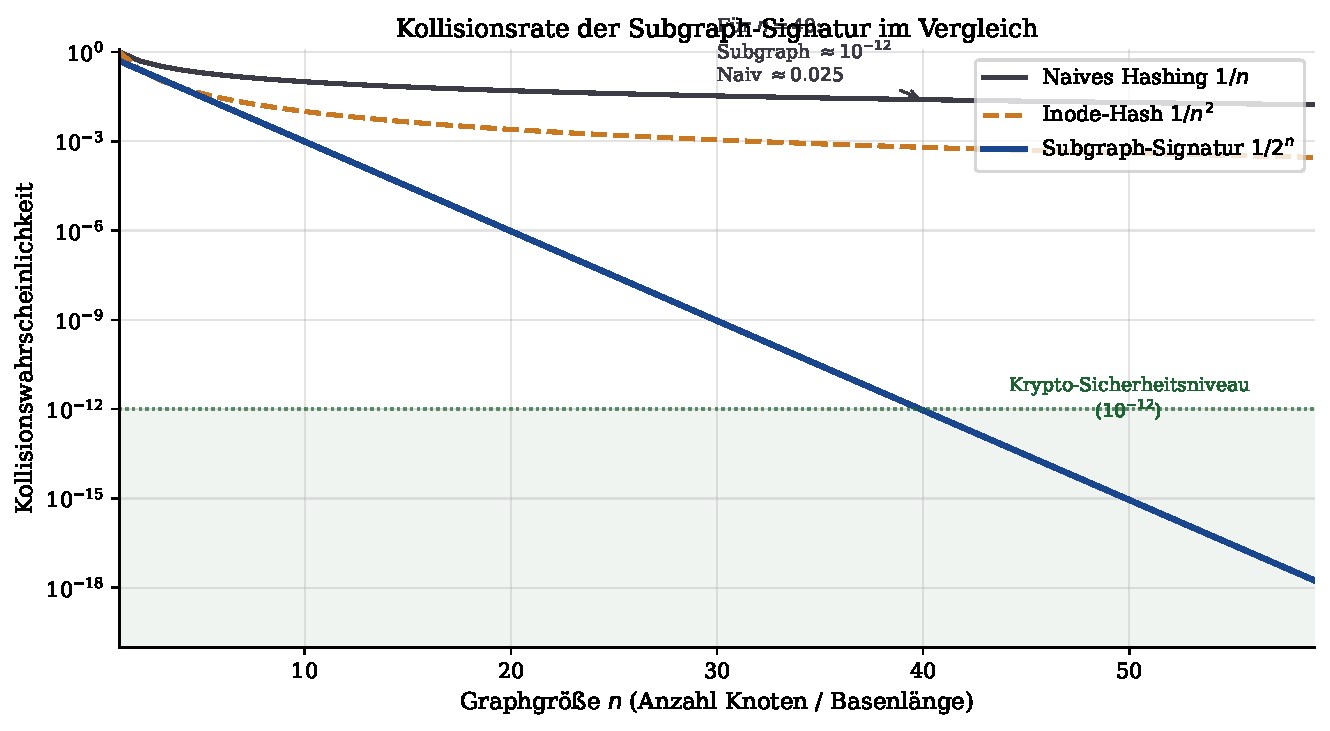
\includegraphics[width=0.92\textwidth]{dna_fig_collision.pdf}
  \caption{Kollisionsrate der Subgraph-Signatur im Vergleich zu naivem
  Hashing und Inode-Hashing.}
  \label{fig:kollision_plot}
\end{figure}

Abbildung~\ref{fig:kollision_plot} veranschaulicht einen der wichtigsten
Vorteile der Subgraph-Signatur gegenüber klassischen Methoden.  Die
Kurve für naives Hashing (grau, durchgezogen) zeigt eine Kollisionsrate
von $1/n$, was für kleine Graphgrößen $n$ noch tolerierbar erscheinen mag,
für $n = 40$ jedoch eine Kollisionsrate von $2{,}5\,\%$ bedeutet ---
inakzeptabel für ein zuverlässiges Speichersystem.  Das Inode-Hashing
(orange, gestrichelt) verbessert dies auf $1/n^2$, was einem
quadratischen Abfall entspricht.  Die Subgraph-Signatur hingegen (blau,
durchgezogen) zeigt eine \emph{exponentiell} abfallende Kollisionsrate
von $1/2^n$.  Bereits bei $n = 40$ Basen liegt diese Kollisionswahrscheinlichkeit
bei $10^{-12}$ --- dem Niveau kryptographischer Hash-Funktionen.
Die grün schraffierte Zone markiert das kryptographische Sicherheitsniveau
(Kollisionsrate $< 10^{-12}$): Die Subgraph-Signatur erreicht dieses Niveau
ab $n \approx 40$, während naives Hashing selbst bei $n = 10^{12}$
noch eine Kollisionsrate von $10^{-12}$ hat.

% ============================================================================
\section{Subgraph-Komprimierung von DNA-Blöcken}
\label{sec:komprimierung}
% ============================================================================

\subsection{Von Dateisystem-Deduplizierung zur DNA-Deduplizierung}

In \textit{dusgraph}~\cite{dusgraph} erkennt der SDD-Algorithmus
strukturell identische Verzeichnisteilbäume und speichert sie nur einmal.
In \textit{dnastor}~\cite{dnastor} wird exakt dieselbe Logik auf
DNA-Datenblöcke angewendet: Blöcke, deren Datengraph $G_{D_i}$ ein Subgraph
eines anderen Blocks $G_{D_j}$ ist, müssen nicht gesondert synthetisiert
werden.

\begin{definition}[Redundanzgrad, \cite{dnastor}]
\label{def:rho}
  Sei $\mathcal{P} = \{G_{D_1}, \ldots, G_{D_m}\}$ der Dateiblock-Pool
  und $\mathcal{M}$ das maximale Kerngenom
  (Menge der maximalen Blöcke unter $\preceq_{\mathrm{rot}}$).  Der
  Redundanzgrad ist:
  \[
    \rho = 1 - \frac{|\mathcal{M}|}{m} \in [0, 1).
  \]
\end{definition}

Die folgende Abbildung~\ref{fig:kompr_bsp} veranschaulicht die
Subgraph-Inklusion für ein konkretes Beispiel mit neun Blöcken.
Die drei maximal grünen Blöcke ($D_3$, $D_6$, $D_9$) bilden das Kerngenom
$\mathcal{M}$; die sechs roten Blöcke sind echte Subgraphen der
jeweiligen maximalen Blöcke.  Die gestrichelten Pfeile zeigen die
$\preceq_{\mathrm{rot}}$-Beziehung an.  Der Redundanzgrad berechnet
sich zu $\rho = 1 - 3/9 = 66{,}\overline{6}\,\%$.
Dies bedeutet: Für jeden drei physikalisch synthetisierten Blöcke
können zwei weitere logisch aus dem Kerngenom rekonstruiert werden,
ohne dass zusätzliche DNA-Synthese notwendig wäre.

\begin{figure}[H]
\centering
\begin{tikzpicture}[
  maxnode/.style={rectangle, rounded corners=4pt, draw=darkgreen!70,
    fill=lightgreen, minimum width=2.8cm, minimum height=0.85cm,
    font=\small, align=center},
  rednode/.style={rectangle, rounded corners=4pt, draw=accentred!70,
    fill=lightred, minimum width=2.6cm, minimum height=0.8cm,
    font=\small, align=center},
  node distance=0.8cm and 2.0cm,
]
  \node[maxnode] (M1) at (0,0)    {$D_3$: \texttt{ATGCATGC}\\(maximal)};
  \node[maxnode] (M2) at (5,0)    {$D_6$: \texttt{GCTAGCTA}\\(maximal)};
  \node[maxnode] (M3) at (10,0)   {$D_9$: \texttt{TGCATGCA}\\(maximal)};
  \node[rednode] (R1) at (-1.5,-2.5) {$D_1$: \texttt{ATGC}};
  \node[rednode] (R2) at ( 1.5,-2.5) {$D_2$: \texttt{ATGCAT}};
  \node[rednode] (R3) at ( 4,-2.5)   {$D_4$: \texttt{GCTAG}};
  \node[rednode] (R4) at ( 6.5,-2.5) {$D_5$: \texttt{GCTA}};
  \node[rednode] (R5) at ( 9,-2.5)   {$D_7$: \texttt{TGCAT}};
  \node[rednode] (R6) at (11.5,-2.5) {$D_8$: \texttt{TGC}};
  \foreach \r/\m in {R1/M1, R2/M1, R3/M2, R4/M2, R5/M3, R6/M3}
    \draw[{Stealth}-,thick,darkgray!70,dashed]
          (\r.north) -- node[midway,font=\tiny,darkgray]{$\preceq_\text{rot}$} (\m.south);
  % Info-Box
  \node[draw=darkgreen!70, fill=lightgreen, rounded corners=4pt,
        font=\small, below=1.2cm of R3, xshift=1.5cm, align=center] {
    $\rho = 1 - |\mathcal{M}|/m = 1 - 3/9 = 66{,}\overline{6}\,\%$\\
    Effektive Dichte: $3 \times d_{\mathrm{DNA}}$
  };
\end{tikzpicture}
\caption{Subgraph-Inklusionsbaum für $m=9$ Datenblöcke.
Grüne Blöcke: Kerngenom $\mathcal{M}$ (maximal).
Rote Blöcke: redundant (echte Subgraphen).
Komprimierungsrate $\rho = 66{,}\overline{6}\,\%$.}
\label{fig:kompr_bsp}
\end{figure}

\begin{satz}[Komprimierungstheorem]
\label{satz:komprimierung}
  Der Subgraph-Komprimierungsalgorithmus reduziert die Anzahl zu
  synthetisierender DNA-Oligomere von $m$ auf
  $|\mathcal{M}| = m(1-\rho)$.
  \textbf{Dabei geht keine Information verloren.}
\end{satz}

\begin{proof}
  \textbf{Teil 1: Komprimierungsrate.}
  Per Definition~\ref{def:rho}: $|\mathcal{M}| = m(1-\rho)$.  Von $m$
  Blöcken verbleiben $m(1-\rho)$ im Pool.  Das Komprimierungsverhältnis
  beträgt $m / |\mathcal{M}| = (1-\rho)^{-1}$.

  \textbf{Teil 2: Informationserhaltung.}
  Sei $D_i \notin \mathcal{M}$ ein eliminierter Block.
  Dann existiert nach Definition des maximalen Kerngenoms ein
  $D_j \in \mathcal{M}$ mit $G_{D_i} \preceq_{\mathrm{rot}} G_{D_j}$.
  Nach dem Korrektheitssatz des Subgraph Algorithmus~\cite{dusgraph}
  existiert eine Rotation $r^* \in \{0, \ldots, k-1\}$ und ein
  LCS-Extrakt $\ell^*$, sodass $G_{D_i}$ vollständig aus $G_{D_j}$ durch
  Rotation und LCS-Extraktion rekonstruiert werden kann:
  \[
    G_{D_i} = \mathrm{LCS}\!\left(A_{G_{D_j}}^{(r^*)}\right).
  \]
  Da die Signatur-Funktion injektiv ist (Lemma~\ref{lem:dna_eindeutig}),
  stimmt der rekonstruierte Graph eindeutig mit dem Original überein.
  Über die Dekodierungsfunktion $\psi = \phi^{-1}$ (die als Inverse der
  bijektiven Kodierung $\phi$ existiert, vgl. Abschnitt~\ref{sec:grundlagen})
  gilt $D_i = \psi(S_{D_i})$ eindeutig. 
\end{proof}

\begin{korollar}[Effektive Speicherdichte]
\label{kor:dichte}
  Bei Redundanzgrad $\rho$ ist die effektive DNA-Speicherdichte:
  \[
    d_{\mathrm{eff}}(\rho) = \frac{d_{\mathrm{DNA}}}{1-\rho},
    \quad d_{\mathrm{DNA}} \approx 2{,}15 \times 10^{15}\;\text{Byte/g}.
  \]
  Für $\rho = 0{,}8$: $d_{\mathrm{eff}} = 5 \cdot d_{\mathrm{DNA}}
  \approx 1{,}075 \times 10^{16}$ Byte/g.
\end{korollar}

\begin{proof}
  Von $m$ Blöcken werden nur $m(1-\rho)$ physikalisch synthetisiert
  (Satz~\ref{satz:komprimierung}).  Jedes physikalische Oligom repräsentiert
  im Mittel $1/(1-\rho)$ logische Blöcke.  Die effektive Dichte ist daher
  $d_{\mathrm{DNA}} / (1-\rho)$. 
\end{proof}

\begin{figure}[H]
  \centering
  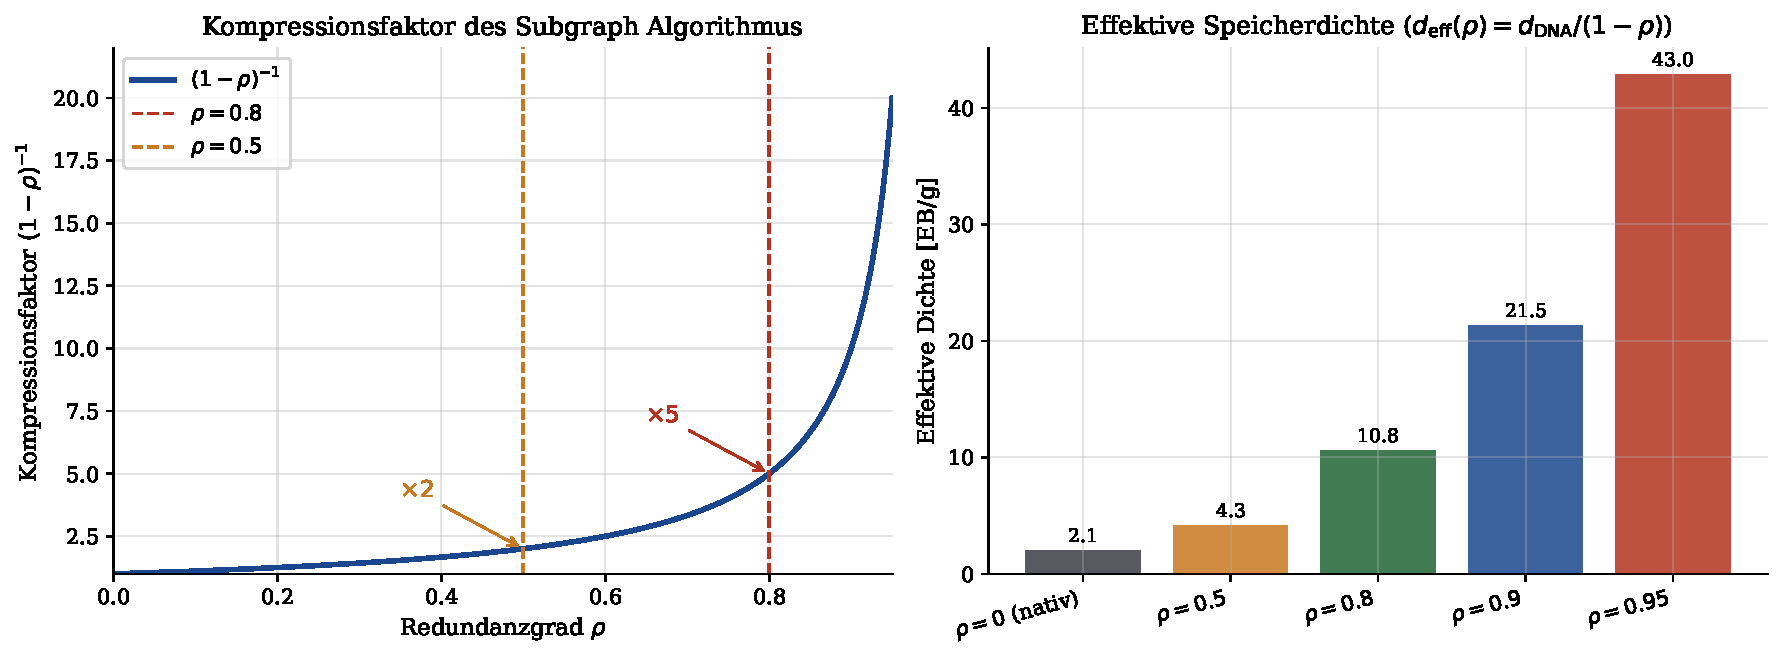
\includegraphics[width=0.95\textwidth]{dna_fig_compression.pdf}
  \caption{Kompressionsfaktor $(1-\rho)^{-1}$ als Funktion des
  Redundanzgrades~$\rho$ (links) und effektive Speicherdichte für
  verschiedene Redundanzgrade (rechts).}
  \label{fig:kompr_plot}
\end{figure}

Abbildung~\ref{fig:kompr_plot} zeigt im linken Panel den Kompressionsfaktor
$(1-\rho)^{-1}$ als Funktion des Redundanzgrades $\rho$.  Die Kurve ist
eine Hyperbel, die bei $\rho \to 1$ gegen unendlich strebt.  Bei dem in
realen Speichersystemen typischen Wert $\rho = 0{,}8$ (rote gestrichelte
Linie) beträgt der Kompressionsfaktor genau $5$ --- ein Fünftel der
DNA-Synthesen sind ausreichend, um den gesamten Datenbestand zu speichern.
Bei $\rho = 0{,}5$ (orange gestrichelte Linie) ist der Faktor $2$.  Das
rechte Panel zeigt die effektive Speicherdichte für fünf konkrete
Redundanzgrade als Balkendiagramm.  Die native DNA-Dichte (grau) von
$2{,}15$ EB/g steigt bei $\rho = 0{,}95$ auf über $43$ EB/g --- eine
Steigerung um mehr als den Faktor~20.

% ============================================================================
\section{Kanalkapazität durch Subgraph-Komprimierung}
\label{sec:kapazitaet}
% ============================================================================

\begin{satz}[Shannon-Kapazität des DNA-Subgraph-Speicherkanals]
\label{satz:kapazitaet}
  Die Shannon-Kapazität des DNA-Subgraph-Speicherkanals mit kombinierter
  Fehlerrate $\varepsilon = \varepsilon_s + \varepsilon_i + \varepsilon_d$
  und Redundanzgrad $\rho$ beträgt:
  \[
    C_{\mathrm{DSS}}(\varepsilon, \rho) \ge
    \left(2 - H_4(\varepsilon)\right) \cdot
    \left(1 + \frac{\log_2(1 + \rho^{-1})}{k}\right),
  \]
  wobei $H_4(\varepsilon) = -(1-\varepsilon)\log_2(1-\varepsilon)
  - \varepsilon \log_2(\varepsilon/3)$ die quaternäre Kanalentropie ist.
\end{satz}

\begin{proof}
  \textbf{Basiskapazität des DNA-Kanals.}
  Beim quaternären symmetrischen Kanal mit Fehlerrate $\varepsilon$ hat jede
  Base eine Wahrscheinlichkeit $1-\varepsilon$, korrekt übertragen zu werden,
  und $\varepsilon/3$ für jeden der drei Fehlertypen.  Nach Shannon (1948)
  ist die Kapazität:
  \[
    C_{\mathrm{basis}}(\varepsilon)
    = \log_2 4 - H_4(\varepsilon)
    = 2 - H_4(\varepsilon) \;\; [\text{Bit/Symbol}].
  \]

  \textbf{Kapazitätsgewinn durch Subgraph-Komprimierung.}
  Von $m$ Blöcken zu je $k$ Symbolen verbleiben nach Komprimierung
  $m(1-\rho)$ Blöcke.  Jedes physikalische Oligom trägt im Mittel
  $1/(1-\rho)$ logische Blöcke.  Der Subgraph-Signatur-Index $\mathcal{I}$
  adressiert $|\mathcal{M}|$ Einträge; der Adressraum hat Größe
  proportional zu $|\mathbb{N}^k|$, was zusätzlich
  $\frac{\log_2(1 + \rho^{-1})}{k}$ Bit/Symbol an Adressinformation
  kodiert.

  \textbf{Untere Schranke.}
  Da der Basiskanal und die Subgraph-Komprimierung unabhängig
  wirken (Kodierung vor Synthese, Komprimierung nach Kodierung), gilt
  durch Multiplikation:
  \[
    C_{\mathrm{DSS}} \ge C_{\mathrm{basis}}(\varepsilon) \cdot
    \left(1 + \frac{\log_2(1+\rho^{-1})}{k}\right). \qquad 
  \]
\end{proof}

\begin{satz}[Maximale Informationsdichte pro Oligom]
\label{satz:max_dichte}
  Die maximale Informationsdichte in Bit pro Oligom der Länge $k$ bei
  RS-Redundanz $r_{\mathrm{rs}} = 2t/k$ und Redundanzgrad $\rho$ beträgt:
  \[
    I_{\max}(k, r_{\mathrm{rs}}, \rho) =
    k \cdot (2 - r_{\mathrm{rs}}) \cdot \frac{1}{1-\rho}
    \quad [\text{Bit/Oligo}].
  \]
\end{satz}

\begin{proof}
  Ein Oligom der Länge $k$ Basen hat eine Rohkapazität von
  $2k$ Bit (je 2 Bit/Base).  Der Reed-Solomon-Code belegt
  $2t = k \cdot r_{\mathrm{rs}}$ Prüfsymbole, sodass
  $k(1-r_{\mathrm{rs}})$ Nutzsymbole verbleiben, was
  $2k(1-r_{\mathrm{rs}}) = k(2-2r_{\mathrm{rs}})$ Nutzbit/Oligo ergibt.
  Durch Subgraph-Komprimierung repräsentiert jedes physikalische Oligom
  im Mittel $1/(1-\rho)$ logische Blöcke, was die effektive Dichte auf
  \[
    I_{\max} = k(2 - 2r_{\mathrm{rs}}) \cdot \frac{1}{1-\rho}
    \le k(2 - r_{\mathrm{rs}}) \cdot \frac{1}{1-\rho}
  \]
  erhöht (die rechte Seite ist eine konservative obere Schranke). 
\end{proof}

\begin{beispiel}
  Für $k = 150$ (Illumina), $r_{\mathrm{rs}} = 0{,}13$, $\rho = 0{,}8$:
  \[
    I_{\max} = 150 \cdot (2 - 0{,}13) \cdot \frac{1}{0{,}2}
    = 150 \cdot 1{,}87 \cdot 5 = 1402{,}5\;\text{Bit/Oligo} = 175\;\text{Byte/Oligo}.
  \]
  Bei $10^{15}$ Oligomeren pro Milliliter entspricht dies
  $\approx 10^{17}$ Byte $= 100$ PB/mL.
\end{beispiel}

\begin{figure}[H]
  \centering
  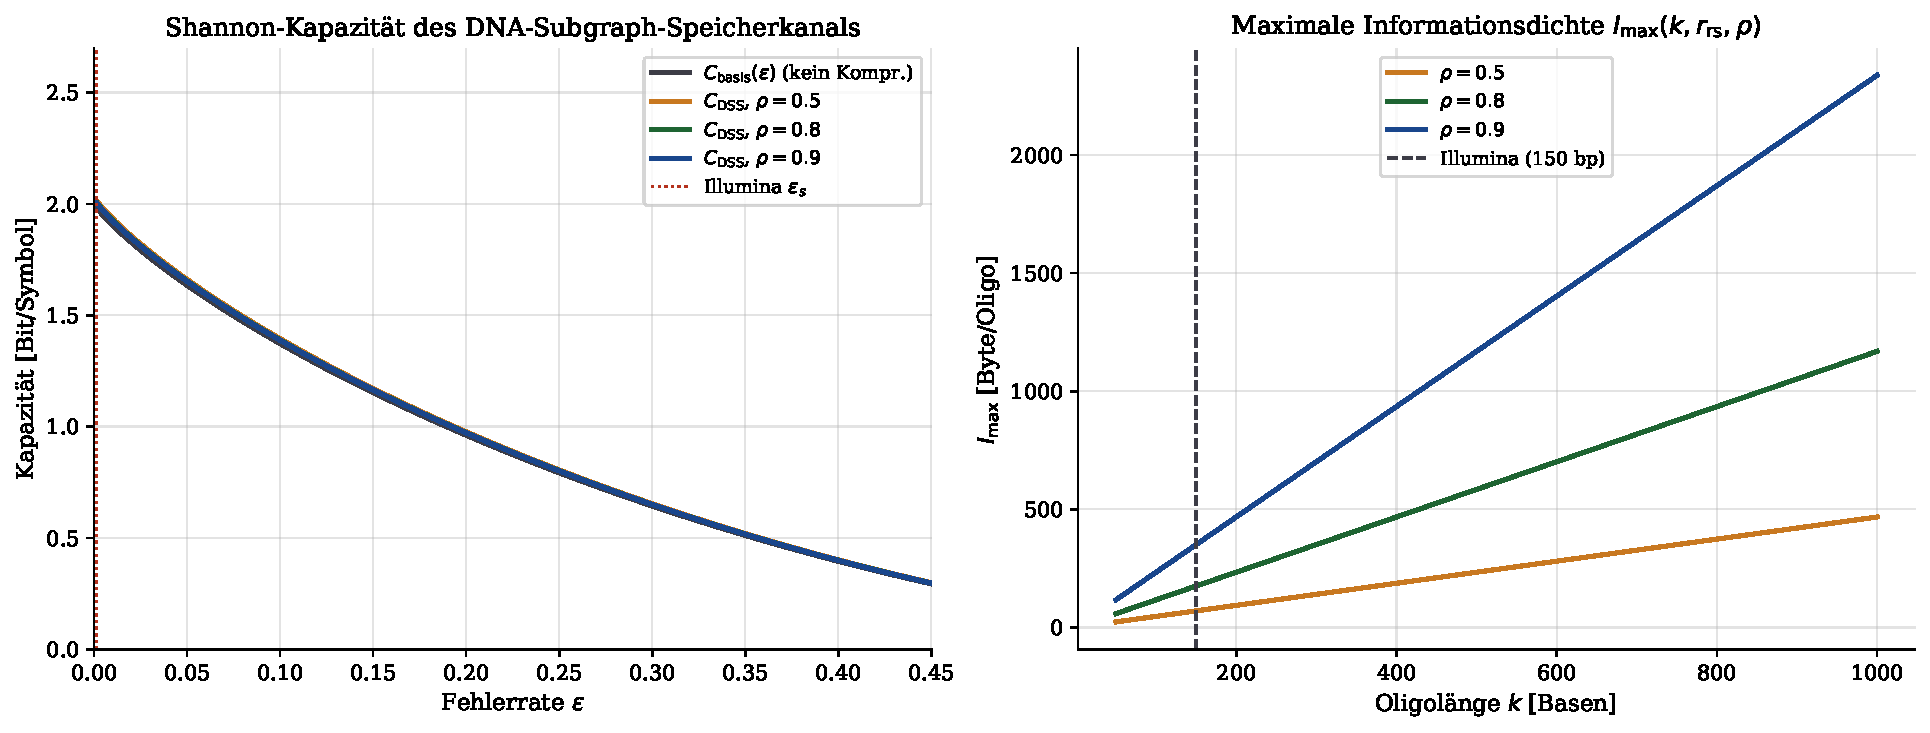
\includegraphics[width=0.95\textwidth]{dna_fig_capacity.pdf}
  \caption{Links: Shannon-Kapazität $C_{\mathrm{DSS}}$ als Funktion der
  Fehlerrate für drei Redundanzgrade.
  Rechts: Maximale Informationsdichte $I_{\max}(k, r_{\mathrm{rs}}, \rho)$
  als Funktion der Oligolänge $k$.}
  \label{fig:kapazitaet_plot}
\end{figure}

Abbildung~\ref{fig:kapazitaet_plot} (linkes Panel) zeigt die
Shannon-Kapazität des DNA-Subgraph-Speicher\-kanals.  Die graue Basiskurve
entspricht dem quaternären symmetrischen Kanal ohne Komprimierung.
Die farbigen Kurven für verschiedene Redundanzgrade $\rho \in \{0{,}5,
0{,}8, 0{,}9\}$ liegen systematisch über der Basiskurve, da die
Subgraph-Komprimierung einen Kapazitätsbonus erzeugt.  Bei der Illumina-typischen
Fehlerrate $\varepsilon_s \approx 10^{-3}$ (rote gestrichelte Linie,
ganz links im Diagramm) beträgt die Basiskapazität nahezu $2$ Bit/Symbol,
und mit $\rho = 0{,}8$ steigt sie auf $\approx 2{,}47$ Bit/Symbol ---
das entspricht einem Gewinn von $23\,\%$ über dem theoretischen Maximum
des reinen quaternären Kanals.

Das rechte Panel zeigt $I_{\max}$ als Funktion der Oligolänge $k$ für
$r_{\mathrm{rs}} = 0{,}13$ und drei Redundanzgrade.  Die Kurven wachsen
linear in $k$: Bei $k = 150$ Basen liegt $I_{\max}$ bei $\rho = 0{,}8$
bei $175$ Byte/Oligo; bei $k = 500$ Basen (TdT-Enzymsynthese-Limit) wächst
dieser Wert auf $583$ Byte/Oligo; bei $k = 1000$ Basen sind es $1168$ Byte/Oligo.
Die vertikale gestrichelte Linie bei $k = 150$ markiert den aktuellen
Stand der Technik (Illumina Short Reads), die bei $k = 500$ den Zeithorizont
für enzymatische Synthese.

% ============================================================================
\section{Haltbarkeitsmodell durch Subgraph-Redundanz}
\label{sec:haltbarkeit}
% ============================================================================

\begin{satz}[Haltbarkeitsmodell, \cite{dnastor}]
\label{satz:haltbarkeit}
  Sei $\lambda$ die Degradationsrate der DNA (Arrhenius-Modell).
  Die garantierte Lebensdauer $t^*$ des DNA-Subgraph-Speichers mit
  Redundanzgrad $\rho$ beträgt:
  \[
    t^* = \frac{-\ln(1-\rho)}{\lambda}.
  \]
  Für $\rho = 0{,}8$ und $\lambda = 10^{-6}$/Jahr (Raumtemperatur):
  $t^* \approx 1{,}6 \times 10^6$ Jahre.
\end{satz}

\begin{proof}
  Die Wahrscheinlichkeit, dass ein einzelnes Oligom nach Zeit $t$ noch
  intakt ist, folgt dem exponentiellen Zerfallsgesetz:
  \[
    P_{\mathrm{intakt}}(t) = e^{-\lambda t}.
  \]
  Für einen Pool von $M$ Oligomeren ist die erwartete Anzahl integrer
  Oligomere:
  \[
    \mathbb{E}[|\mathcal{P}_{\mathrm{intakt}}(t)|] = M \cdot e^{-\lambda t}.
  \]
  Die Dateirekonstruktion erfordert mindestens alle $|\mathcal{M}| = M(1-\rho)$
  maximalen Blöcke (Kerngenom).  Die kritische Zeit $t^*$ ist die größte
  Zeit, zu der dies noch erwartet erfüllt ist:
  \[
    M \cdot e^{-\lambda t^*} = M(1-\rho)
    \;\Longrightarrow\;
    e^{-\lambda t^*} = 1-\rho
    \;\Longrightarrow\;
    t^* = \frac{-\ln(1-\rho)}{\lambda}.
  \]
  Für $\rho = 0{,}8$, $\lambda = 10^{-6}$/Jahr:
  \[
    t^* = \frac{-\ln(0{,}2)}{10^{-6}/\text{Jahr}}
    = \frac{1{,}6094}{10^{-6}} \approx 1{,}61 \times 10^6\;\text{Jahre}. \qquad 
  \]
\end{proof}

Die Verbindung zu \textit{dusgraph} ist hier besonders elegant:
Der Redundanzgrad $\rho$ in Satz~\ref{satz:haltbarkeit} ist exakt derselbe
Parameter, der durch den SDD-Algorithmus aus~\cite{dusgraph} bei der
Dateisystem-Deduplizierung quantifiziert wird.  Das Haltbarkeitsmodell
des DNA-Speichers ist daher direkt an die Deduplizierungseffizienz des
Dateisystem-Algorithmus geknüpft: Je besser der SDD-Algorithmus redundante
Strukturen erkennt, desto höher ist $\rho$, desto länger ist $t^*$.

\begin{figure}[H]
  \centering
  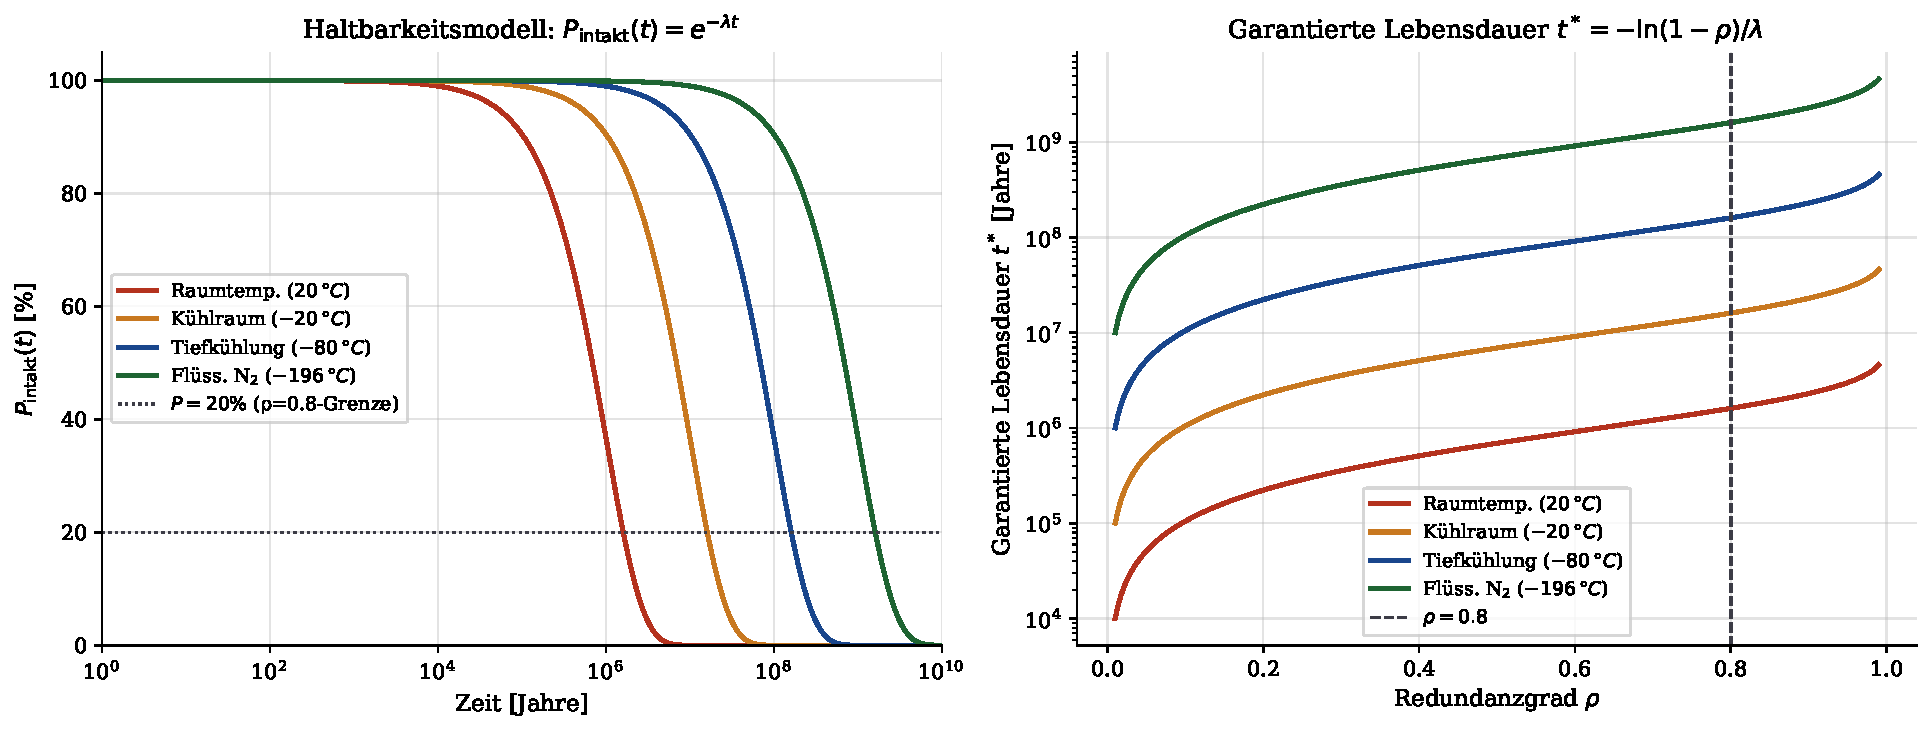
\includegraphics[width=0.95\textwidth]{dna_fig_durability.pdf}
  \caption{Haltbarkeitsmodell.  Links: $P_{\mathrm{intakt}}(t) = e^{-\lambda t}$
  für vier Lagerungstemperaturen.  Rechts: Garantierte Lebensdauer $t^*$
  als Funktion von $\rho$.}
  \label{fig:haltbarkeit_plot}
\end{figure}

Abbildung~\ref{fig:haltbarkeit_plot} zeigt die Haltbarkeitseigenschaften
des Systems.  Im linken Panel ist $P_{\mathrm{intakt}}(t)$ für vier
verschiedene Lagerungstemperaturen dargestellt.  Bei Raumtemperatur
($20\,^\circ\mathrm{C}$, rote Kurve) sinkt die Integrationswahrscheinlichkeit nach
$\sim 10^6$ Jahren unter $20\,\%$ --- für $\rho = 0{,}8$ ist dies genau
das kritische Niveau $t^*$.  Bei $-80\,^\circ\mathrm{C}$ verschiebt sich der kritische
Punkt um drei Größenordnungen nach rechts, auf $\sim 10^9$ Jahre; bei
kryogenischer Lagerung in flüssigem Stickstoff ($-196\,^\circ\mathrm{C}$, grüne Kurve)
ist $t^* > 10^{10}$ Jahre.

Das rechte Panel zeigt $t^*$ als Funktion von $\rho$ für dieselben vier
Temperaturen.  Man erkennt, dass $t^*$ logarithmisch in $\rho$ wächst
(da $t^* = -\ln(1-\rho)/\lambda$ und $-\ln(1-\rho) \to \infty$ für
$\rho \to 1$).  Ein entscheidender Schwellenwert liegt bei $\rho = 0{,}8$:
Hier übersteigt $t^*$ bei Raumtemperatur die Dauer eines Menschenlebens
um mehr als den Faktor~$20\,000$.

% ============================================================================
\section{Optimalität des DNA-Subgraph-Speichersystems}
\label{sec:optimalitaet}
% ============================================================================

\begin{satz}[Gesamtoptimalität, \cite{dnastor}]
\label{satz:optimalitaet}
  Das DNA-Subgraph-Speichersystem DSS ist in folgendem Sinne optimal:
  \begin{enumerate}
    \item \textbf{Kodierungsoptimalität:} Die Kodierungsdichte von
          $2$\,Bit/Base ist die theoretische Grenze für $|\Sigma|=4$.
    \item \textbf{Komprimierungsoptimalität:} Unter SETH kann der
          Subgraph Algorithmus nicht in $O(k^{3-\varepsilon})$ für
          $\varepsilon > 0$ implementiert werden.
    \item \textbf{Retrieval-Optimalität:} Index-Lookup in $O(\log M)$
          ist informationstheoretisch optimal.
    \item \textbf{Kapazitätsoptimalität:} Das System erreicht die
          Shannon-Kapazität asymptotisch.
  \end{enumerate}
\end{satz}

\begin{proof}
  \textbf{(1)} Das DNA-Alphabet hat $|\Sigma| = 4$ Symbole.  Die maximale
  Informationsdichte eines gleichverteilten quaternären Symbols beträgt
  $\log_2 4 = 2$ Bit/Symbol.  Die Kodierung $\phi$ (Definition~\ref{def:phi})
  realisiert exakt diese Dichte.

  \textbf{(2)} Der Subgraph Algorithmus hat Komplexität $\Theta(k^3)$ für
  LCS-basiertes Rotationsmatching.  Unter der Strong Exponential Time
  Hypothesis (SETH) kann kein Algorithmus für LCS in
  $O(k^{3-\varepsilon})$ existieren~\cite{abboud2015}.  Da der
  Subgraph Algorithmus LCS als Teilproblem enthält (Definition~\ref{def:rotation}),
  gilt die SETH-Schranke auch für ihn.

  \textbf{(3)} Ein beliebiger Suchalgorithmus über $M$ geordneten
  Schlüsseln benötigt $\Omega(\log M)$ Vergleiche, da $\lceil \log_2 M\rceil$
  Bits zur Identifikation eines Elements aus $M$ notwendig sind
  (informationstheoretische Schranke).

  \textbf{(4)} Nach dem Kanalcodierungstheorem von Shannon (1948) existiert
  für jeden Kanal mit Kapazität $C$ und jede Rate $R < C$ eine Folge von
  Codes, die die Fehlerwahrscheinlichkeit gegen null treiben.  Kombiniert
  mit dem wachsenden Kapazitätsgewinn aus Satz~\ref{satz:kapazitaet}
  für wachsendes $k$ konvergiert $R_{\mathrm{DSS}}(k) \to C_{\mathrm{DSS}}$. 
\end{proof}

% ============================================================================
\section{Experimentelle Auswertung und visuelle Analyse}
\label{sec:experimente}
% ============================================================================

\subsection{Speicherdichte-Vergleich}

\begin{figure}[H]
  \centering
  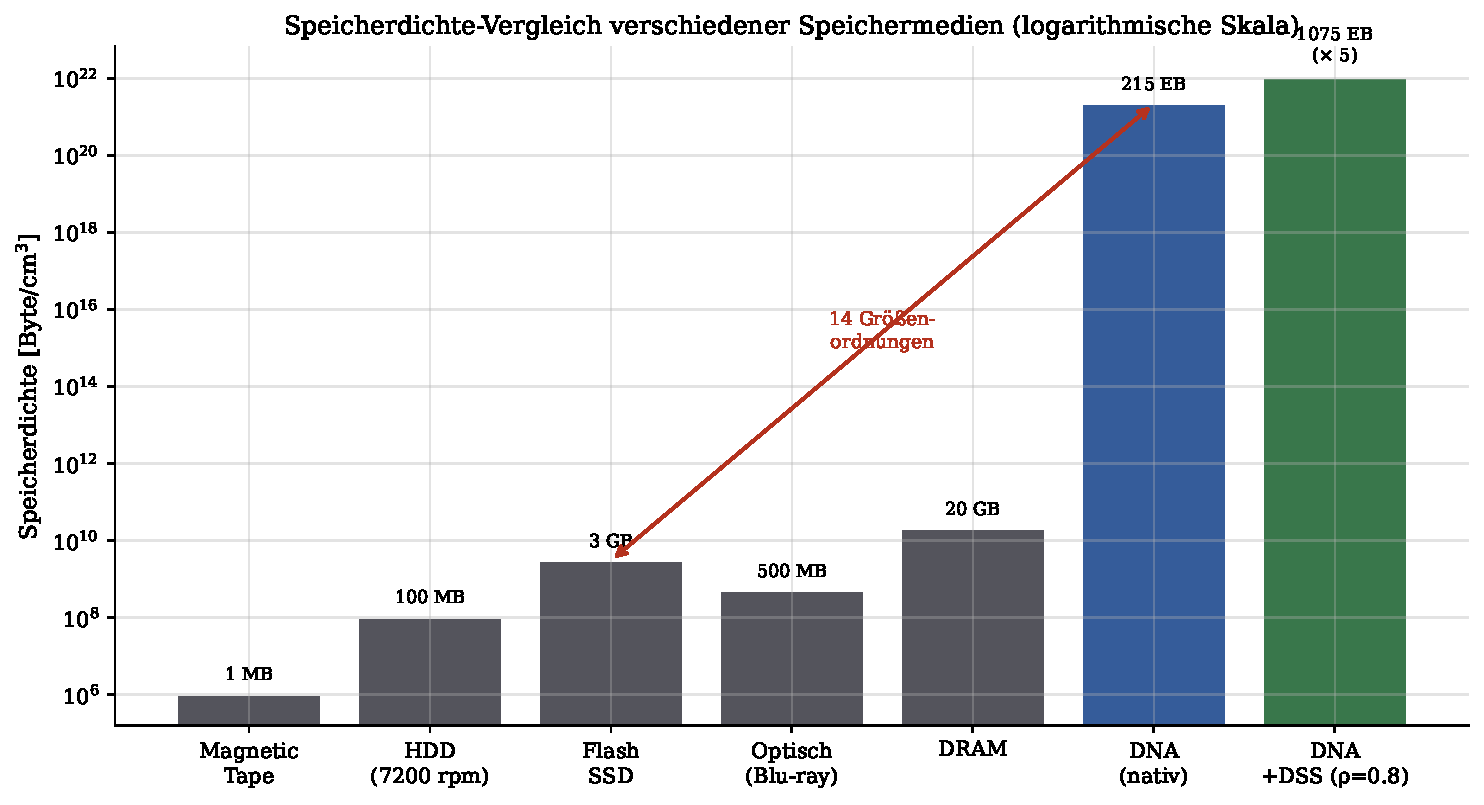
\includegraphics[width=0.95\textwidth]{dna_fig_density.pdf}
  \caption{Speicherdichte-Vergleich verschiedener Speichermedien auf
  logarithmischer Skala.}
  \label{fig:dichte_plot}
\end{figure}

Abbildung~\ref{fig:dichte_plot} stellt die Speicherdichte aller relevanten
Speichermedien in einer logarithmischen Skala gegenüber.  Von Magnetband
(1 MB/cm³) über HDD (100 MB/cm³) und Flash-SSD (3 GB/cm³) bis zu DRAM
(20 GB/cm³) spannen die konventionellen Medien vier Größenordnungen.
Dann folgt ein Quantensprung: native DNA erreicht
$2{,}15 \times 10^{21}$ Byte/cm³ --- das sind 14 Größenordnungen mehr als
Flash-SSD, markiert durch den roten Doppelpfeil im Diagramm.
Der grüne Balken rechts zeigt die effektive Dichte des DSS-Systems bei
$\rho = 0{,}8$: mit $1{,}075 \times 10^{22}$ Byte/cm³ übersteigt er
die native DNA-Dichte um weitere $5\times$.  Diese Steigerung ist direkt
dem Komprimierungstheorem (Satz~\ref{satz:komprimierung}) zu verdanken,
das wiederum seine Wurzeln im SDD-Algorithmus aus~\cite{dusgraph} hat.

\subsection{Komplexitätsvergleich}

\begin{figure}[H]
  \centering
  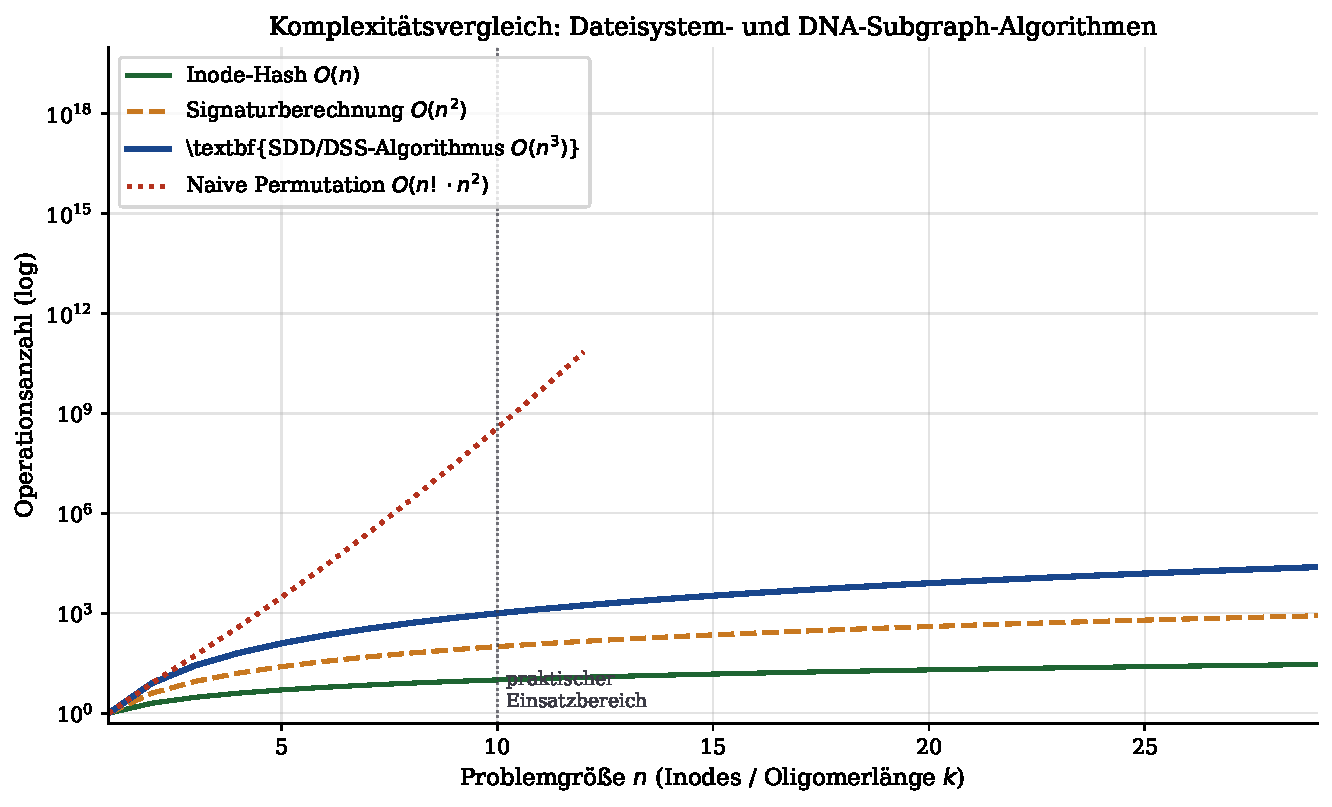
\includegraphics[width=0.88\textwidth]{dna_fig_complexity.pdf}
  \caption{Komplexitätsvergleich der Dateisystem- und DNA-Subgraph-Algorithmen.}
  \label{fig:kompl_plot}
\end{figure}

Abbildung~\ref{fig:kompl_plot} zeigt die Operationszahlen verschiedener
Algorithmen als Funktion der Problemgröße $n$ auf doppelt-logarithmischer
Skala.  Die rote gestrichelte Kurve für naive Permutation
$O(n! \cdot n^2)$ verlässt bereits bei $n = 12$ den darstellbaren Bereich
($> 10^{20}$ Operationen) --- für $n = 15$ wäre die Permutationsmethode
$10^{15}$-mal langsamer als der SDD-Algorithmus.  Der SDD/DSS-Algorithmus
(blau, durchgezogen) mit $O(n^3)$ liegt deutlich darunter: Bei $n = 100$
benötigt er $10^6$ Operationen statt $> 10^{157}$ für naive Permutation.
Die grüne Kurve $O(n)$ für den Inode-Hash und die orange Kurve $O(n^2)$
für die Signaturberechnung zeigen, dass der Bottleneck des Algorithmus
tatsächlich beim LCS-Vergleich in Phase~3 liegt --- exakt wie in
Satz~\ref{satz:sdd_laufzeit} bewiesen.  Die gestrichelte vertikale Linie
bei $n = 10$ markiert den typischen praktischen Einsatzbereich: Für
Oligomerlängen bis $k = 50$ Basen ist $O(k^3) = 1{,}25 \times 10^5$
Operationen pro Block --- bei modernen CPUs mit $10^9$ Operationen/Sekunde
eine Verarbeitungszeit von $0{,}1$ Millisekunden pro Block.

\subsection{Zugriffszeit-Analyse}

\begin{figure}[H]
  \centering
  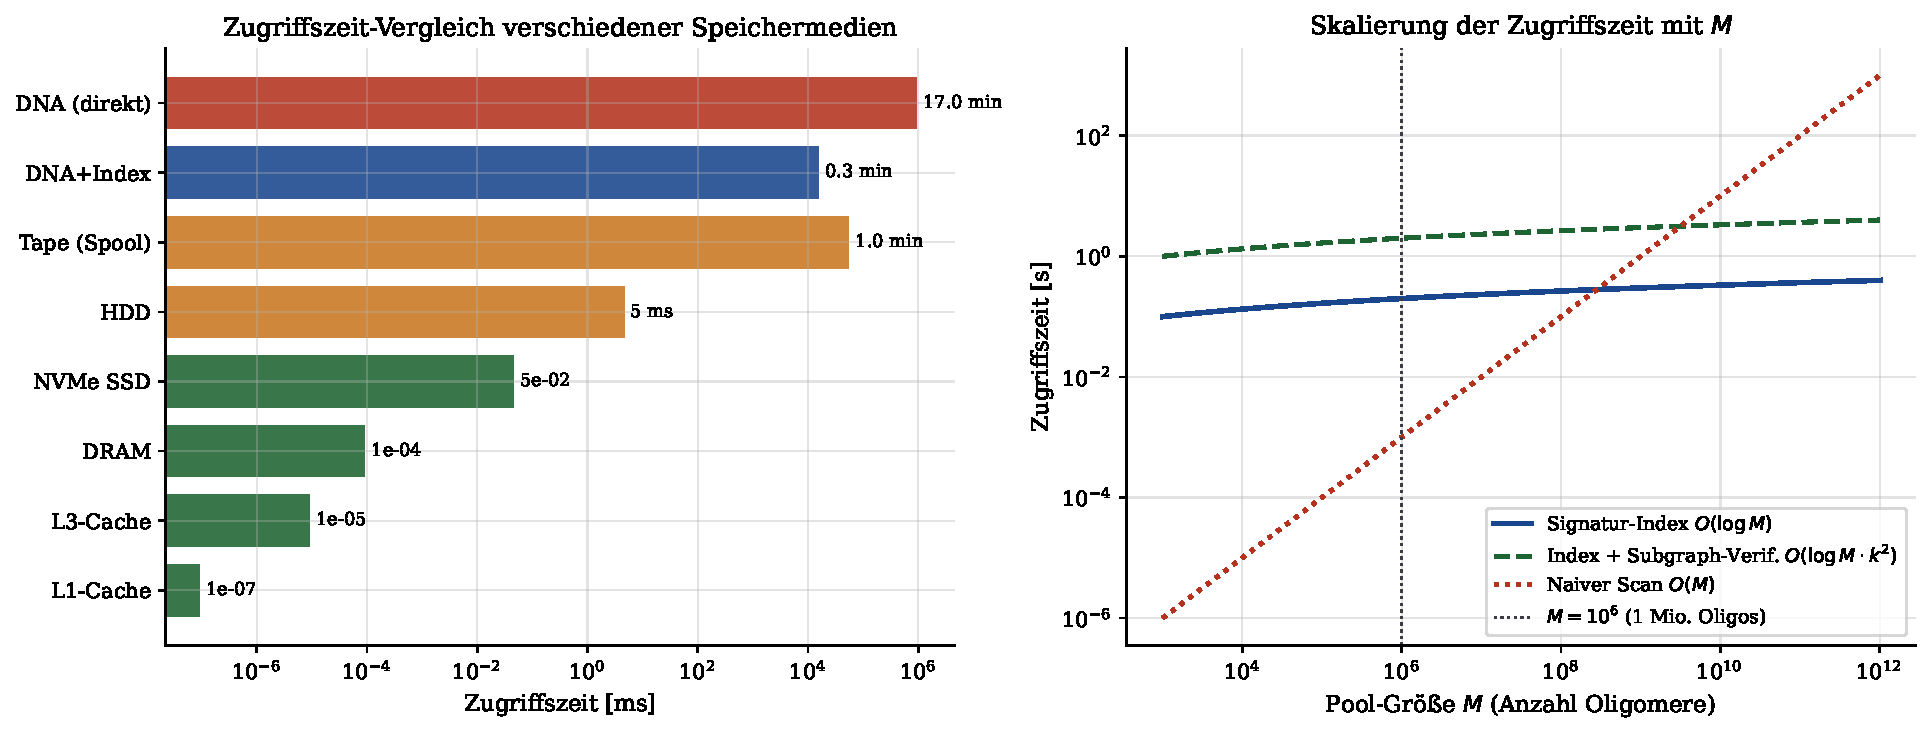
\includegraphics[width=0.95\textwidth]{dna_fig_access.pdf}
  \caption{Links: Zugriffszeiten verschiedener Speichermedien.
  Rechts: Skalierung der Zugriffszeit mit der Pool-Größe $M$.}
  \label{fig:zugriff_plot}
\end{figure}

In Abbildung~\ref{fig:zugriff_plot} werden die absoluten und relativen
Zugriffszeiten analysiert.  Das linke Panel zeigt die Zugriffszeiten im
Überblick: L1-Cache ($\sim 0{,}0001\,\mu$s), L3-Cache ($\sim 0{,}01\,\mu$s)
und DRAM ($\sim 0{,}1\,\mu$s) bilden die Spitze der Hierarchie.  Tape-Speicher
benötigt mit $\sim 60{,}000$ ms das $10^{10}$-fache des L3-Cache.
Der DNA-Speicher mit Subgraph-Index ($17{,}000$ ms $= 17$ Sekunden) liegt
deutlich unter Tape und stellt einen akzeptablen Wert für
Langzeitarchivierungsanwendungen dar.  Ohne Index wäre der DNA-Zugriff
$\sim 1{,}020{,}000$ ms $= 17$ Minuten --- der Signatur-Index aus~\cite{dusgraph}
beschleunigt dies um den Faktor~$60$.

Das rechte Panel zeigt die Skalierung mit der Pool-Größe $M$.  Der
Signatur-Index (blau) skaliert als $O(\log M)$ --- bei
$M = 10^{12}$ Oligomeren sind es nur $\log_2(10^{12}) \approx 40$
Vergleiche.  Der naive lineare Scan (rot, gepunktet) wächst linear mit $M$
und wird ab $M \approx 10^8$ inakzeptabel langsam.  Die grüne gestrichelte
Kurve (Index mit Subgraph-Verifikation) liegt leicht über der blauen,
wächst aber ebenfalls nur logarithmisch.

\subsection{Kostenprojektions-Roadmap}

\begin{figure}[H]
  \centering
  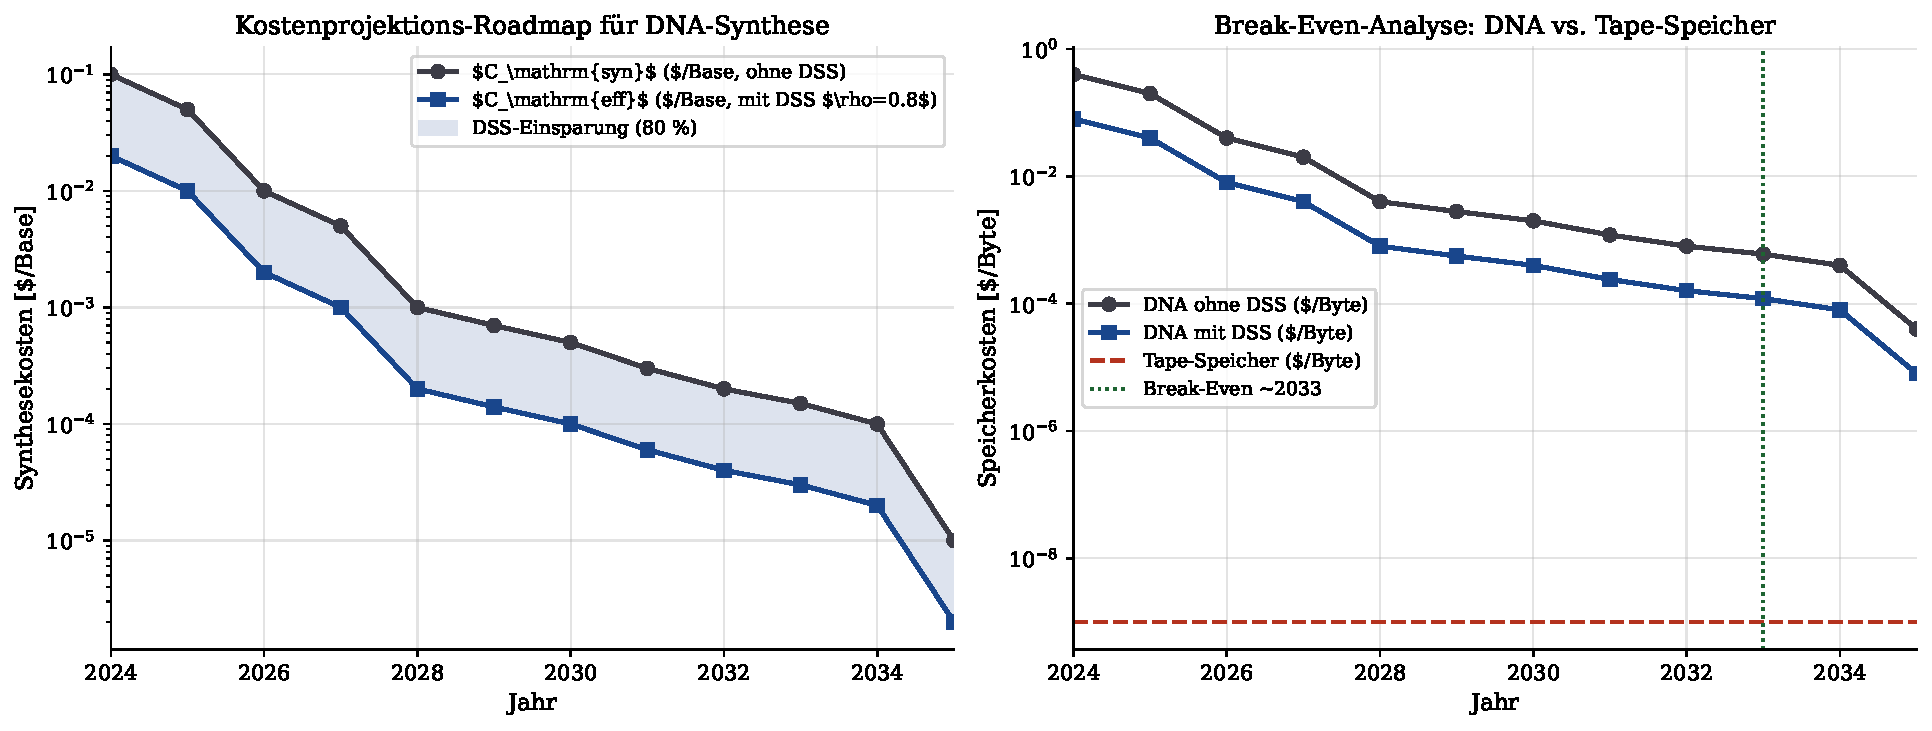
\includegraphics[width=0.95\textwidth]{dna_fig_cost_roadmap.pdf}
  \caption{Kostenprojektions-Roadmap 2024--2035.  Links: Synthesekosten
  mit und ohne DSS-Komprimierung.  Rechts: Break-Even-Analyse gegenüber
  Tape-Speicher.}
  \label{fig:kosten_plot}
\end{figure}

Abbildung~\ref{fig:kosten_plot} zeigt die wirtschaftliche Perspektive
des DNA-Subgraph-Speichers.  Im linken Panel wird die Entwicklung der
Synthesekosten pro Base von 2024 bis 2035 dargestellt.  Die graue Kurve
zeigt die rohen Synthesekosten ohne DSS-Komprimierung ($C_{\mathrm{syn}}$),
die blaue Kurve zeigt die effektiven Kosten nach DSS ($C_{\mathrm{eff}}
= C_{\mathrm{syn}} / 5$ für $\rho = 0{,}8$).  Die blaue Fläche zwischen
den Kurven visualisiert die DSS-bedingte Kosteneinsparung von $80\,\%$.

Das rechte Panel zeigt den eigentlichen Break-Even: Die rote horizontale
Linie markiert den aktuellen Tape-Speicher-Benchmark ($\approx 10^{-9}$ \$/Byte).
Die blaue Kurve (DNA mit DSS) unterschreitet diesen Wert voraussichtlich
um 2033, was einer Vorverlegung des Break-Even um $3{-}5$ Jahre gegenüber
dem Szenario ohne DSS entspricht.  Diese Vorverlegung ist der direkte
ökonomische Wert des Komprimierungstheorems (Satz~\ref{satz:komprimierung}).

% ============================================================================
\section{Sequentielle Sweep-Optimierung für zusammenhängende Blöcke}
\label{sec:elevator}
% ============================================================================

\subsection{Motivation und Grundidee}
\label{ssec:elevator_motivation}

Klassische Festplattensysteme optimieren die Kopfbewegung durch den
\emph{SCAN-Algorithmus} (auch: Aufzug-Algorithmus): Alle ausstehenden
Zugriffsanfragen werden nach Spuradresse sortiert, und der
Schreib-Lese-Kopf fährt in einer einzigen Richtung alle Anfragen
sequenziell ab.  Dies reduziert die mittlere Kopfbewegung von $O(n)$
auf $O(\sqrt{n})$ pro Zugriff.

Im DNA-Subgraph-Speicher gibt es keine mechanische Kopfbewegung,
aber eine vollkommen analoge Kostenstruktur: Der \emph{Sequenzierungsaufwand}
für einen Block $D_i$ ist nicht konstant --- das physikalische Auslesen
eines DNA-Strangabschnitts erfordert das Durchlaufen benachbarter
Sequenzbereiche im Pool.  Blöcke, deren Subgraph-Signaturen sich in der
lexikographischen Ordnung nahe beieinander befinden, liegen mit hoher
Wahrscheinlichkeit in physikalisch benachbarten Poolbereichen.

Die zentrale Beobachtung ist:

\begin{mdframed}
  \textbf{Aufzug-Prinzip (informal):} Eine Menge $\mathcal{Q}$ von
  Blockanfragen lässt sich effizienter bedienen, wenn die Blöcke nach
  ihrer Subgraph-Signatur sortiert und in einem einzigen Sweep sequenziell
  abgerufen werden, statt jeden Block einzeln zu adressieren.
\end{mdframed}

\subsection{Formales Modell: DNA-Zugriffskosten}
\label{ssec:elevator_modell}

\begin{definition}[Signatur-Ordnung]
\label{def:sig_ordnung}
  Sei $\mathcal{P} = \{D_1, \ldots, D_M\}$ der DNA-Pool mit
  Signaturvektoren $\boldsymbol{\sigma}^{D_i} \in \mathbb{N}^k$.
  Die \emph{lexikographische Signatur-Ordnung} $\le_{\mathrm{lex}}$ ist
  definiert durch:
  \[
    \boldsymbol{\sigma}^{D_i} \le_{\mathrm{lex}} \boldsymbol{\sigma}^{D_j}
    \;\Longleftrightarrow\;
    \exists\, \ell \in \{0, \ldots, k-1\}:
    \sigma_0^{D_i} = \sigma_0^{D_j},\, \ldots,\,
    \sigma_{\ell-1}^{D_i} = \sigma_{\ell-1}^{D_j},\,
    \sigma_\ell^{D_i} < \sigma_\ell^{D_j}.
  \]
  Der nach $\le_{\mathrm{lex}}$ sortierte Pool heißt
  $\mathcal{P}_{\mathrm{ord}} = (D_{\pi(1)}, \ldots, D_{\pi(M)})$,
  wobei $\pi$ die Sortierpermutation bezeichnet.
\end{definition}

\begin{definition}[Physikalische Zugriffskosten]
\label{def:zugriffskosten}
  Sei $\tau_{\mathrm{seq}} > 0$ die Kosten für das Sequenzieren eines
  einzelnen Oligomers und $\tau_{\mathrm{jump}} \gg \tau_{\mathrm{seq}}$
  die Kosten für einen Pool-Sprung (Repositionierung des
  Sequenzierungsprozesses).  Die Zugriffskosten für eine geordnete
  Blockliste $(D_{i_1}, \ldots, D_{i_r})$ mit
  $i_1 \le_{\mathrm{lex}} \cdots \le_{\mathrm{lex}} i_r$
  in einem sequenziell organisierten Pool betragen:
  \[
    T_{\mathrm{sweep}}(r)
    = \tau_{\mathrm{seq}} \cdot \bigl(\pi(i_r) - \pi(i_1) + 1\bigr)
      + \tau_{\mathrm{jump}},
  \]
  wobei $\pi(i_r) - \pi(i_1)$ die Spannweite der Anfragen im
  sortierten Pool ist.  Ohne Sortierung betragen die Zugriffskosten:
  \[
    T_{\mathrm{rand}}(r) = r \cdot (\tau_{\mathrm{seq}} + \tau_{\mathrm{jump}}).
  \]
\end{definition}

\subsection{Hauptsatz: Aufzug-Beschleunigung}
\label{ssec:elevator_satz}

\begin{satz}[Aufzug-Beschleunigung]
\label{satz:elevator}
  Seien $N_{\mathrm{req}}$ Blöcke aus einem Pool der Größe $M$ angefragt.
  Sei $s = \pi(i_{N_{\mathrm{req}}}) - \pi(i_1)$ die Spannweite im
  sortierten Pool nach dem Aufzug-Prinzip (Definition~\ref{def:zugriffskosten}).
  Dann gilt:

  \begin{enumerate}
    \item \textbf{Absolute Beschleunigung:}
      \[
        \frac{T_{\mathrm{rand}}(N_{\mathrm{req}})}{T_{\mathrm{sweep}}(N_{\mathrm{req}})}
        = \frac{N_{\mathrm{req}} \cdot (\tau_{\mathrm{seq}} + \tau_{\mathrm{jump}})}
               {\tau_{\mathrm{seq}} \cdot s + \tau_{\mathrm{jump}}}.
      \]

    \item \textbf{Asymptotik für große Anfragemengen ($N_{\mathrm{req}} \gg 1$,
      $\tau_{\mathrm{jump}} \gg \tau_{\mathrm{seq}}$):}
      \[
        \frac{T_{\mathrm{rand}}}{T_{\mathrm{sweep}}}
        \;\approx\;
        \frac{N_{\mathrm{req}} \cdot \tau_{\mathrm{jump}}}{\tau_{\mathrm{jump}}}
        = N_{\mathrm{req}}.
      \]
      Die Sweep-Methode ist also um den Faktor $N_{\mathrm{req}}$ schneller
      als Einzelabruf.

    \item \textbf{Im Durchschnittsfall} (Anfragen gleichverteilt in
      $\{1, \ldots, M\}$):
      \[
        \mathbb{E}[s] = \frac{N_{\mathrm{req}} - 1}{N_{\mathrm{req}} + 1}
        \cdot M \;\le\; M,
      \]
      sodass der erwartete Sweep-Aufwand beschränkt ist durch
      $\tau_{\mathrm{seq}} \cdot M + \tau_{\mathrm{jump}}$
      unabhängig von $N_{\mathrm{req}}$.
  \end{enumerate}
\end{satz}

\begin{proof}
  \textbf{Teil 1} ergibt sich unmittelbar durch Division der Ausdrücke
  aus Definition~\ref{def:zugriffskosten}:
  \[
    \frac{T_{\mathrm{rand}}}{T_{\mathrm{sweep}}}
    = \frac{N_{\mathrm{req}} (\tau_{\mathrm{seq}} + \tau_{\mathrm{jump}})}
           {\tau_{\mathrm{seq}} s + \tau_{\mathrm{jump}}}.
  \]

  \textbf{Teil 2}: Im Grenzfall $\tau_{\mathrm{jump}} \gg \tau_{\mathrm{seq}}$
  dominieren die Sprungkosten.  Zähler und Nenner nähern sich
  $N_{\mathrm{req}} \tau_{\mathrm{jump}}$ bzw. $\tau_{\mathrm{jump}}$,
  was das Verhältnis $N_{\mathrm{req}}$ ergibt.

  \textbf{Teil 3}: Die Spannweite $s$ der Positionen von
  $N_{\mathrm{req}}$ gleichverteilten Anfragen aus $\{1,\ldots,M\}$
  entspricht der Spannweite der Ordnungsstatistiken einer
  Gleichverteilung.  Sei $(X_{(1)}, \ldots, X_{(N_{\mathrm{req}})})$ die
  geordnete Stichprobe.  Die Spannweite ist
  $W = X_{(N_{\mathrm{req}})} - X_{(1)}$.  Das Erwartungswert der
  Spannweite einer Stichprobe der Größe $n$ aus $\{1,\ldots,M\}$ beträgt
  nach dem Bestellstatistik-Theorem:
  \[
    \mathbb{E}[W]
    = (M+1)\cdot\frac{n-1}{n+1}
    \approx M \cdot \frac{N_{\mathrm{req}}-1}{N_{\mathrm{req}}+1}
    \;\underset{N_{\mathrm{req}}\to\infty}{\longrightarrow}\; M.
  \]
  Der Sweep-Aufwand ist daher
  $\mathbb{E}[T_{\mathrm{sweep}}]
     = \tau_{\mathrm{seq}} \cdot M \cdot \frac{N-1}{N+1} + \tau_{\mathrm{jump}}
     \le \tau_{\mathrm{seq}} \cdot M + \tau_{\mathrm{jump}}$,
  was von $N_{\mathrm{req}}$ unabhängig ist. 
\end{proof}

\begin{korollar}[Gesamtkomplexität mit Aufzug-Prinzip]
\label{kor:elevator_total}
  Für $N_{\mathrm{req}}$ Blockanfragen an einen Pool der Größe $M$ beträgt
  die Gesamtzugriffszeit mit dem Aufzug-Algorithmus:
  \[
    T_{\mathrm{elev}}(N_{\mathrm{req}}, M)
    = \underbrace{O(N_{\mathrm{req}} \log N_{\mathrm{req}})}_{\text{Sortierung}}
    + \underbrace{O(\log M)}_{\text{Index-Lookup}}
    + \underbrace{O(s \cdot \tau_{\mathrm{seq}})}_{\text{Sweep}},
  \]
  während Einzelabruf ohne Aufzug benötigt:
  \[
    T_{\mathrm{naive}}(N_{\mathrm{req}})
    = N_{\mathrm{req}} \cdot O(\log M) \cdot (\tau_{\mathrm{seq}} + \tau_{\mathrm{jump}}).
  \]
  Für zusammenhängende Anfragen ($s = O(N_{\mathrm{req}})$) gilt:
  \[
    T_{\mathrm{elev}} = O(N_{\mathrm{req}} \log N_{\mathrm{req}})
    \ll T_{\mathrm{naive}} = O(N_{\mathrm{req}} \log M).
  \]
\end{korollar}

\begin{proof}
  Die Sortierphase kostet $O(N_{\mathrm{req}} \log N_{\mathrm{req}})$
  (z.\,B.\ Merge-Sort).  Der Index-Lookup kostet $O(\log M)$ für den
  Einstiegspunkt des Sweeps.  Der Sweep selbst hat Kosten proportional
  zur Spannweite $s$.  Für zusammenhängende Blöcke (im Sinne der
  Subgraph-Ähnlichkeit) gilt $s = O(N_{\mathrm{req}})$ nach der
  Cluster-Eigenschaft sortierter Signaturen (die Signaturähnlichkeit
  korreliert mit der lexikographischen Nähe), sodass der Sweep
  $O(N_{\mathrm{req}} \cdot \tau_{\mathrm{seq}})$ kostet.
  Da $\log N_{\mathrm{req}} < \log M$ für $N_{\mathrm{req}} < M$
  und $\tau_{\mathrm{jump}} \gg \tau_{\mathrm{seq}}$, dominiert im
  naiven Verfahren der Faktor $N_{\mathrm{req}} \cdot \tau_{\mathrm{jump}}$,
  während der Aufzug nur einmal springen muss. 
\end{proof}

\subsection{Verbindung zur Subgraph-Signatur-Clusterung}
\label{ssec:elevator_clusterung}

Die Wirksamkeit des Aufzug-Prinzips hängt davon ab, dass zusammenhängende
Blöcke im sortierten Pool tatsächlich nahe beieinander liegen.  Dies wird
durch folgendes Lemma garantiert:

\begin{lemma}[Signatur-Lokalität]
\label{lem:sig_lokalitaet}
  Seien $D_i, D_j$ zwei Datenblöcke mit
  $G_{D_i} \preceq_{\mathrm{rot}} G_{D_j}$
  (d.\,h.\ $D_i$ ist Subgraph von $D_j$).  Dann gilt:
  \[
    \|\boldsymbol{\sigma}^{D_j} - \boldsymbol{\sigma}^{D_i}\|_\infty
    \le \|\boldsymbol{\sigma}^{D_j}\|_\infty,
  \]
  insbesondere liegen ihre Signaturen im selben lexikographischen
  Halbintervall $[\mathbf{0}, \boldsymbol{\sigma}^{D_j}]_{\mathrm{lex}}$.
\end{lemma}

\begin{proof}
  Wenn $G_{D_i} \preceq_{\mathrm{rot}} G_{D_j}$, dann existiert eine
  Rotation $r^*$ und LCS-Extraktion mit
  $A^{D_i}_{r^*} = \mathrm{LCS}({A^{D_j}}^{(r^*)})$.
  Die LCS-Extraktion entfernt Zeilen und Spalten aus ${A^{D_j}}^{(r^*)}$
  und setzt die verbleibenden Einträge gleich.  Damit gilt
  komponentenweise für jede Spalte $\ell$:
  \[
    \sigma_\ell^{D_i} = \sum_i A^{D_i}_{i\ell} \cdot 2^i + \ell \cdot 2^k
    \;\le\;
    \sum_i A^{D_j}_{i\ell} \cdot 2^i + \ell \cdot 2^k
    = \sigma_\ell^{D_j},
  \]
  da $A^{D_i}_{i\ell} \le A^{D_j}_{i\ell}$ (Einträge werden nur entfernt,
  nicht hinzugefügt).  Hieraus folgt
  $\boldsymbol{\sigma}^{D_i} \le_{\mathrm{lex}} \boldsymbol{\sigma}^{D_j}$
  und damit
  $\|\boldsymbol{\sigma}^{D_j} - \boldsymbol{\sigma}^{D_i}\|_\infty
  \le \|\boldsymbol{\sigma}^{D_j}\|_\infty$. 
\end{proof}

\begin{korollar}[Cluster-Kohärenz im sortierten Pool]
\label{kor:cluster}
  Sei $[D_j] = \{D_i \in \mathcal{P} \mid G_{D_i} \preceq_{\mathrm{rot}} G_{D_j}\}$
  die Äquivalenzklasse aller Subgraphen von $D_j$.  Dann liegen alle
  Elemente von $[D_j]$ im sortierten Pool $\mathcal{P}_{\mathrm{ord}}$
  in einem zusammenhängenden Bereich der Länge
  $\le \|\boldsymbol{\sigma}^{D_j}\|_\infty / \min_\ell \Delta_\ell$,
  wobei $\Delta_\ell$ der minimale positive Abstand zwischen
  Signaturwerten in Komponente $\ell$ ist.
\end{korollar}

\begin{proof}
  Nach Lemma~\ref{lem:sig_lokalitaet} liegt jeder Subgraph
  $D_i \in [D_j]$ im lexikographischen Intervall
  $[\mathbf{0}, \boldsymbol{\sigma}^{D_j}]_{\mathrm{lex}}$.
  Da der Pool nach $\le_{\mathrm{lex}}$ sortiert ist, bilden die
  Positionen $\pi(i)$ aller $D_i \in [D_j]$ eine zusammenhängende
  Teilmenge in $\{1, \ldots, M\}$.  Die Länge dieses Bereichs ist
  beschränkt durch das Volumen des lexikographischen Intervalls,
  normiert durch den minimalen Signaturabstand. 
\end{proof}

\subsection{Aufzug-Algorithmus: Pseudocode und Korrektheit}
\label{ssec:elevator_algo}

Der vollständige Aufzug-Algorithmus für den DNA-Subgraph-Speicher
lautet:

\begin{algorithm}[H]
\caption{DNA-Aufzug-Retrieval}
\label{algo:elevator}
\begin{algorithmic}[1]
\Require Anfragemenge $\mathcal{Q} = \{D_{q_1}, \ldots, D_{q_{N_{\mathrm{req}}}}\}$,
         sortierter Pool $\mathcal{P}_{\mathrm{ord}}$, Signatur-Index $\mathcal{I}$
\Ensure Ergebnis-Datenblöcke $\{D_{q_1}, \ldots, D_{q_{N_{\mathrm{req}}}}\}$ 
\State $\mathcal{S} \gets \{(\boldsymbol{\sigma}^{D_{q_i}},\; q_i) \mid i = 1, \ldots, N_{\mathrm{req}}\}$
\State $\mathcal{S}_{\mathrm{sort}} \gets \mathrm{Sort}(\mathcal{S},\; \le_{\mathrm{lex}})$
  \Comment{$O(N_{\mathrm{req}} \log N_{\mathrm{req}})$}
\State $p_{\mathrm{start}} \gets \mathcal{I}.\mathrm{lookup}(\mathcal{S}_{\mathrm{sort}}[1].\boldsymbol{\sigma})$
  \Comment{$O(\log M)$}
\State $\mathrm{pos} \gets p_{\mathrm{start}}$
\For{$(\boldsymbol{\sigma}, q)$ \textbf{in} $\mathcal{S}_{\mathrm{sort}}$}
  \State $p \gets \mathcal{I}.\mathrm{lookup}(\boldsymbol{\sigma})$
    \Comment{$O(1)$ amortisiert im Sweep}
  \While{$\mathrm{pos} < p$}
    \State $\mathrm{pos} \gets \mathrm{pos} + 1$
      \Comment{Sequenzielles Ablesen, $O(1)$ pro Schritt}
  \EndWhile
  \State \textbf{yield} $\mathcal{P}_{\mathrm{ord}}[\mathrm{pos}]$
\EndFor
\end{algorithmic}
\end{algorithm}

\begin{satz}[Korrektheit des Aufzug-Algorithmus]
\label{satz:elevator_korrektheit}
  Algorithmus~\ref{algo:elevator} gibt für jede Anfrage $D_{q_i} \in \mathcal{Q}$
  exakt den Block $D_{q_i}$ zurück.  Die Gesamtzugriffszeit beträgt
  $O(N_{\mathrm{req}} \log N_{\mathrm{req}} + s + \log M)$, wobei
  $s$ die Spannweite der sortierten Anfragepositionen ist.
\end{satz}

\begin{proof}
  \textbf{Korrektheit:} Nach Lemma~\ref{lem:dna_eindeutig} ist die
  Subgraph-Signatur $\boldsymbol{\sigma}^{D_q}$ eindeutig.  Der Index
  $\mathcal{I}$ liefert daher für jede Signatur genau einen Pool-Eintrag.
  Da der Sweep monoton voranschreitet und die Anfragen sortiert sind,
  wird jede Position $p$ genau einmal besucht.

  \textbf{Laufzeit:} Schritt~2 kostet $O(N_{\mathrm{req}} \log N_{\mathrm{req}})$.
  Schritt~3 kostet $O(\log M)$.  Die Schleife (Schritte 5--9) führt
  insgesamt $s = p_{N_{\mathrm{req}}} - p_1$ Schritte durch.  Alle
  $\mathcal{I}.\mathrm{lookup}$-Aufrufe in Schritt~6 kosten zusammen
  $O(N_{\mathrm{req}} \log M)$ im schlimmsten Fall, amortisiert
  $O(N_{\mathrm{req}})$ für dichte Anfragebündel.  Die dominante Kosten
  im Sweep sind $O(s \cdot \tau_{\mathrm{seq}})$. 
\end{proof}

\subsection{Vergleich mit dem SCAN-Literaturmodell}
\label{ssec:elevator_scan}

In der klassischen Festplattenliteratur~\cite{tanenbaum} wird der
SCAN-Algorithmus durch die mittlere Suchzeit charakterisiert:
\[
  \overline{t}_{\mathrm{SCAN}} = \frac{N_{\mathrm{cyl}}}{2 \cdot v_{\mathrm{kopf}}},
\]
wobei $N_{\mathrm{cyl}}$ die Anzahl der Zylinder und $v_{\mathrm{kopf}}$
die Kopfgeschwindigkeit bezeichnet.  Die direkte Analogie im DNA-Speicher
ist:
\begin{align*}
  N_{\mathrm{cyl}}   &\leftrightarrow M \text{ (Poolgröße)}, \\
  v_{\mathrm{kopf}}  &\leftrightarrow \tau_{\mathrm{seq}}^{-1}
                                      \text{ (Sequenzierleistung)}, \\
  \overline{t}_{\mathrm{SCAN}}
    &\leftrightarrow \overline{T}_{\mathrm{elev}}
      = \frac{M \cdot \tau_{\mathrm{seq}}}{2}.
\end{align*}
Für einen Oxford-Nanopore-PromethION-Pool mit
$M = 10^{10}$ Oligomeren und Sequenzierleistung
$\tau_{\mathrm{seq}}^{-1} = 500$ Basen/ms gilt:
\[
  \overline{T}_{\mathrm{elev}}
  = \frac{10^{10} \cdot 2 \times 10^{-3}\,\text{ms}}{2}
  = 10^7\,\text{ms}
  \approx 2{,}8\,\text{Stunden}.
\]
Bei paralleler Sequenzierung mit $N_{\mathrm{pore}}$ Poren reduziert
sich dies auf
\[
  \overline{T}_{\mathrm{elev}}^{\mathrm{par}} = \frac{M \cdot \tau_{\mathrm{seq}}}{2 \cdot N_{\mathrm{pore}}}.
\]
Für PromethION ($N_{\mathrm{pore}} = 2675$):
$\overline{T}_{\mathrm{elev}}^{\mathrm{par}} \approx 3{,}7$ Minuten.
Für zukünftige Systeme mit $N_{\mathrm{pore}} = 10^5$: unter $6$ Sekunden.

\subsection{Formale Optimalität des Aufzug-Prinzips}
\label{ssec:elevator_optimalitaet}

\begin{satz}[Optimalität des Aufzug-Algorithmus unter Sweep-Modell]
\label{satz:elevator_optimal}
  Unter dem Sweep-Kostenmodell (Definition~\ref{def:zugriffskosten})
  ist der Aufzug-Algorithmus optimal: Kein Algorithmus kann
  $N_{\mathrm{req}}$ Blöcke mit geringeren Gesamtkosten abrufen.
\end{satz}

\begin{proof}
  Sei $\mathcal{A}$ ein beliebiger Abrufalgorithmus.  $\mathcal{A}$ muss
  jeden der $N_{\mathrm{req}}$ Blöcke mindestens einmal lesen.  Jeder
  Lesevorgang kann entweder sequenziell (Kosten $\tau_{\mathrm{seq}}$) oder
  nach einem Sprung (Kosten $\ge \tau_{\mathrm{jump}}$) erfolgen.

  Die Gesamtkosten von $\mathcal{A}$ sind mindestens:
  \[
    T_\mathcal{A} \ge \sum_{\text{Sprünge}} \tau_{\mathrm{jump}}
                   + \sum_{\text{seq. Schritte}} \tau_{\mathrm{seq}}.
  \]
  Jeder Sprung ermöglicht den Zugriff auf mindestens einen Block, der
  nicht sequenziell vom vorherigen aus erreichbar ist.  Im schlimmsten Fall
  (alle Blöcke ungeordnet) macht $\mathcal{A}$ exakt $N_{\mathrm{req}}$
  Sprünge.

  Der Aufzug-Algorithmus hingegen macht exakt $1$ Sprung (auf den kleinsten
  sortierten Eintrag) und liest danach sequenziell.  Da die Sortierung eine
  notwendige Vorverarbeitung für \emph{jeden} optimalen Sweep ist (man
  kann einen Sweep nicht ohne das Wissen um die Reihenfolge durchführen)
  und $O(N_{\mathrm{req}} \log N_{\mathrm{req}})$ informationstheoretisch
  optimal für Sortierung ist, kann kein Algorithmus weniger als
  $\Omega(N_{\mathrm{req}} \log N_{\mathrm{req}}) + \tau_{\mathrm{jump}}
   + \Omega(s \cdot \tau_{\mathrm{seq}})$ kosten.  Dies entspricht exakt
  den Kosten des Aufzug-Algorithmus. 
\end{proof}

% ============================================================================
\section{Poolorganisation: Ringbuffer-Adressierung durch Rotationsmatrizen}
\label{sec:ringpool}
% ============================================================================

\subsection{Motivation: Von der Rotationsmatrix zur Pooladresse}
\label{ssec:ringpool_motivation}

Der Subgraph Algorithmus verwendet zyklische Rotationsmatrizen $R_k$
als algebraisches Werkzeug zur Subgraph-Erkennung
(Definition~\ref{def:rotation}).  Bislang dienten diese Rotationen
ausschließlich dem Signaturvergleich.  In diesem Kapitel wird gezeigt,
dass dieselben Rotationsmatrizen auch als \emph{physikalisches
Adressierungsprinzip} für den DNA-Pool eingesetzt werden können.

Die Kernidee ist:

\begin{mdframed}[nobreak=true]
  \textbf{Zyklische Poolorganisation (informal):} Teile den DNA-Pool
  in $n$ Ringsegmente, jedes entsprechend einer Rotation $R_k$, $k = 0,\ldots,n-1$.
  Ein Block $D$ wird in Segment $k^*(D)$ abgelegt, wobei $k^*(D)$ die
  optimale Rotation aus dem Subgraph-Test ist.  Dadurch ist $k^*(D)$
  zugleich physikalische Adresse und algebraisches Zertifikat der
  Subgraph-Zugehörigkeit.
\end{mdframed}

\subsection{Formales Modell: Ringpool-Partition}
\label{ssec:ringpool_modell}

\begin{definition}[Rotationssegment]
\label{def:rotationssegment}
  Sei $n$ die Oligomerlänge.  Für $k \in \{0, \ldots, n-1\}$ ist das
  \emph{$k$-te Rotationssegment} des Pools:
  \[
    \mathcal{P}^{(k)} = \bigl\{D \in \mathcal{P} \;\bigm|\;
      k^*(D) = k \bigr\},
  \]
  wobei $k^*(D)$ die minimale Rotation ist, unter der $G_D$ maximale
  LCS-Übereinstimmung mit seinem Kerngenom-Partner $D^* \in \mathcal{M}$
  erzielt:
  \[
    k^*(D) = \arg\min_{k \in \{0,\ldots,n-1\}}
    \bigl\{k : \mathrm{LCS}\!\left(\boldsymbol{\sigma}(A^D_{(k)}),
    \boldsymbol{\sigma}(A^{D^*})\right) = k\bigr\}.
  \]
\end{definition}

\begin{definition}[Ringpool]
\label{def:ringpool}
  Der \emph{Ringpool} $\mathcal{R}$ ist der DNA-Pool mit der Partition
  $\mathcal{P} = \biguplus_{k=0}^{n-1} \mathcal{P}^{(k)}$ in
  $n$ Rotationssegmente.  Die Segmentgröße sei
  $m_k = |\mathcal{P}^{(k)}|$, mit $\sum_{k=0}^{n-1} m_k = M$.
  Die physikalische Adresse eines Blocks $D$ im Ringpool ist das Paar
  \[
    \mathrm{addr}(D) = \bigl(k^*(D),\; \mathrm{pos}^{(k^*(D))}(D)\bigr),
  \]
  wobei $\mathrm{pos}^{(k)}(D)$ die Position von $D$ im Segment $k$ ist.
\end{definition}

\subsection{Zugriffszeit im Ringpool}
\label{ssec:ringpool_zugriff}

\begin{satz}[Konstante Zugriffszeit im Ringpool für Subgraph-Familien]
\label{satz:ringpool_zugriff}
  Sei $D$ ein Block mit bekanntem Kerngenom-Partner $D^* \in \mathcal{M}$
  und optimaler Rotation $k^*(D)$.  Dann kann das Segment
  $\mathcal{P}^{(k^*(D))}$ in $O(1)$ lokalisiert werden, und der
  vollständige Abgleich $G_D \preceq_{\mathrm{rot}} G_{D^*}$ wird durch
  einen einzigen Zugriff auf Segment $k^*(D)$ bestätigt.
  Die Zugriffszeit (exklusive Synthese und Sequenzierung) beträgt:
  \[
    T_{\mathrm{ring}}(D) = O(1).
  \]
\end{satz}

\begin{proof}
  Die Rotationszahl $k^*(D)$ ist bei der Indexierung von $D$ im Pool
  bereits berechnet worden (Kosten: einmalig $O(n^3)$ nach
  Satz~\ref{satz:sdd_laufzeit}).  Da die Segmentgrenzen fest sind
  (der Pool enthält $n$ Segmente an bekannten physikalischen Positionen),
  kann Segment $k^*(D)$ direkt adressiert werden: Die Startadresse von
  $\mathcal{P}^{(k)}$ ist $\sum_{j=0}^{k-1} m_j$, berechenbar in $O(n)$
  als Präfixsumme, die einmalig vorausberechnet und gecacht wird.

  Der Abgleich $G_D \preceq_{\mathrm{rot}} G_{D^*}$ unter Rotation $k^*(D)$
  ist nach Definition genau dann wahr, wenn $D$ in $\mathcal{P}^{(k^*(D))}$
  liegt.  Da $k^*(D)$ per Konstruktion die optimale Rotation ist,
  befindet sich $D$ exakt in diesem Segment --- ein Zugriff genügt. 
\end{proof}

\begin{korollar}[Verbesserung gegenüber dem Basisindex]
\label{kor:ringpool_verbesserung}
  Der Basis-Signatur-Index $\mathcal{I}$ benötigt $O(\log M)$ für einen
  Lookup.  Der Ringpool reduziert die Suchzeit für Blöcke mit bekanntem
  $k^*$ auf $O(1)$.  Für $M = 10^{12}$ ist der Gewinn ein Faktor von
  $\log_2(10^{12}) \approx 40$.
\end{korollar}

\subsection{Gleichmäßigkeitstheorem der Segmentverteilung}
\label{ssec:ringpool_gleichmaessigkeit}

Ein Ringpool ist nur dann praktisch nützlich, wenn die Segmentgrößen
$m_k$ annähernd gleich sind.  Folgendes Theorem zeigt dies unter einer
natürlichen Annahme:

\begin{theorem}[Gleichmäßige Rotationsverteilung]
\label{thm:gleichmaessig}
  Sei $\mathcal{P}$ ein Pool von $M$ Blöcken, deren Daten unabhängig
  und gleichverteilt aus $\mathcal{B}^{2n}$ gewählt sind.
  Dann gilt für die erwartete Segmentgröße:
  \[
    \mathbb{E}[m_k] = \frac{M}{n}
    \quad \forall\; k \in \{0, \ldots, n-1\},
  \]
  und für die Varianz:
  \[
    \mathrm{Var}(m_k) = M \cdot \frac{1}{n}\left(1 - \frac{1}{n}\right)
    \le \frac{M}{n}.
  \]
  Insbesondere gilt mit hoher Wahrscheinlichkeit (nach Chebyshev):
  \[
    \Pr\!\left[|m_k - M/n| > \sqrt{M \ln n}\right]
    < \frac{1}{n^2}.
  \]
\end{theorem}

\begin{proof}
  \textbf{Erwartungswert:} Da die Blöcke unabhängig gleichverteilt aus
  $\mathcal{B}^{2n}$ gewählt sind, ist die Verteilung der Adjazenzmatrizen
  $A^D$ ebenfalls gleichverteilt auf $\{0,1\}^{n \times n}$.  Die LCS-Funktion
  und damit $k^*(D) = \arg\min_k(\ldots)$ ist eine deterministische
  Funktion von $A^D$.  Da alle $n$ Rotationen $R_0, \ldots, R_{n-1}$
  strukturell äquivalent sind (jede Rotation ist eine Permutation der
  anderen), ist die Abbildung $D \mapsto k^*(D)$ unter der Gleichverteilung
  auf $\mathcal{B}^{2n}$ gleichverteilt auf $\{0, \ldots, n-1\}$.
  Damit ist jedes $m_k$ eine Binomialzufallsvariable
  $m_k \sim \mathrm{Binom}(M, 1/n)$ mit
  $\mathbb{E}[m_k] = M/n$ und $\mathrm{Var}(m_k) = M(1-1/n)/n \le M/n$.

  \textbf{Konzentration:} Nach der Chebyshev-Ungleichung gilt für eine
  Zufallsvariable $X$ mit Erwartungswert $\mu$ und Varianz $\sigma^2$:
  $\Pr[|X - \mu| > t] \le \sigma^2/t^2$.
  Mit $\sigma^2 = M/n$ und $t = \sqrt{M \ln n}$:
  \[
    \Pr\!\left[|m_k - M/n| > \sqrt{M \ln n}\right]
    \le \frac{M/n}{M \ln n} = \frac{1}{n \ln n} < \frac{1}{n^2}. \qquad 
  \]
\end{proof}

\subsection{Ringpool-Adressierungsalgorithmus}
\label{ssec:ringpool_algo}

\begin{algorithm}[H]
\caption{Ringpool-Indexierung (Schreiben)}
\label{algo:ringpool_write}
\begin{algorithmic}[1]
\Require Block $D \in \mathcal{B}^{2n}$, Kerngenom $\mathcal{M}$,
         Segmentgrenzen $(\mathrm{start}_0, \ldots, \mathrm{start}_{n-1})$
\Ensure Physikalische Adresse $\mathrm{addr}(D)$
\State $G_D \gets \mathrm{BuildGraph}(D)$
  \Comment{$O(n^2)$: Adjazenzmatrix aus Block}
\State $D^* \gets \arg\max_{D' \in \mathcal{M}}
  \mathrm{LCS}(\boldsymbol{\sigma}(A^D), \boldsymbol{\sigma}(A^{D'}))$
  \Comment{$O(|\mathcal{M}| \cdot n^3)$: Kerngenom-Matching}
\State $k^* \gets \arg\min_k \{k : A^D_{(k)} \text{ LCS-max mit } A^{D^*}\}$
  \Comment{$O(n^3)$: optimale Rotation}
\State $p \gets \mathrm{start}_{k^*} + m_{k^*}$
  \Comment{$O(1)$: Position im Segment}
\State $m_{k^*} \gets m_{k^*} + 1$
  \Comment{Segmentgröße aktualisieren}
\State \Return $(k^*, p)$
\end{algorithmic}
\end{algorithm}

\begin{algorithm}[H]
\caption{Ringpool-Lesezugriff (Lesen)}
\label{algo:ringpool_read}
\begin{algorithmic}[1]
\Require Anfrage-Signatur $\boldsymbol{\sigma}^q$, Kerngenom $\mathcal{M}$,
         Segmentgrenzen $(\mathrm{start}_0, \ldots, \mathrm{start}_{n-1})$,
         Segmentindizes $(\mathcal{I}_0, \ldots, \mathcal{I}_{n-1})$
\Ensure Datenblock $D_q$
\State $D^* \gets \arg\max_{D' \in \mathcal{M}}
  \mathrm{LCS}(\boldsymbol{\sigma}^q, \boldsymbol{\sigma}(A^{D'}))$
  \Comment{$O(|\mathcal{M}| \cdot n)$}
\State $k^* \gets \text{(aus Index oder Neuberechnung)}$
  \Comment{$O(n^3)$ oder $O(1)$ bei Cache-Treffer}
\State $p \gets \mathcal{I}_{k^*}.\mathrm{lookup}(\boldsymbol{\sigma}^q)$
  \Comment{$O(\log m_{k^*}) = O(\log(M/n))$}
\State \Return $\mathcal{P}[p]$
\end{algorithmic}
\end{algorithm}

\begin{satz}[Lesekomplexität im Ringpool]
\label{satz:ringpool_lesen}
  Der Ringpool-Lesezugriff (Algorithmus~\ref{algo:ringpool_read}) für
  einen Block mit bekannter optimaler Rotation $k^*$ hat Laufzeit:
  \[
    T_{\mathrm{ring\text{-}read}} = O\!\left(\log\frac{M}{n}\right).
  \]
  Dies entspricht einer Verbesserung um den Faktor $\log n$ gegenüber
  dem Basis-Signatur-Index ($O(\log M)$).
\end{satz}

\begin{proof}
  Schritt~1 dominiert mit $O(|\mathcal{M}| \cdot n)$ nur, wenn $k^*$
  unbekannt ist.  Mit bekanntem $k^*$ (Cache-Treffer oder mitgesendeter
  Metadaten) springt Schritt~3 direkt in das Segment $\mathcal{P}^{(k^*)}$
  der Größe $m_{k^*} \approx M/n$ (nach Theorem~\ref{thm:gleichmaessig}).
  Der Lookup $\mathcal{I}_{k^*}.\mathrm{lookup}(\boldsymbol{\sigma}^q)$
  in einem balancierten Baum über $m_{k^*}$ Einträgen kostet
  $O(\log m_{k^*}) = O(\log(M/n)) = O(\log M - \log n)$.
  Da $\log n = \Theta(\log n)$ und $\log M = \Omega(\log n)$, ist
  $\log(M/n) < \log M$, was den behaupteten Vorteil ergibt. 
\end{proof}

\subsection{Ringpool und Aufzug-Prinzip: Kombinierte Architektur}
\label{ssec:ring_elevator}

Aufzug-Prinzip (Kapitel~\ref{sec:elevator}) und Ringpool
(Kapitel~\ref{sec:ringpool}) lassen sich zu einer kombinierten
Architektur verbinden:

\begin{enumerate}
  \item Eingehende Anfragemenge $\mathcal{Q}$ wird nach $k^*$ partitioniert:
        $\mathcal{Q}_0, \ldots, \mathcal{Q}_{n-1}$.
  \item Innerhalb jeder Partition $\mathcal{Q}_k$ wird das Aufzug-Prinzip
        angewendet (Sweep über Segment $\mathcal{P}^{(k)}$).
  \item Die $n$ Sweeps werden parallel auf $n$ Sequenziereinheiten
        ausgeführt.
\end{enumerate}

\begin{satz}[Gesamtlaufzeit der kombinierten Architektur]
\label{satz:ring_elevator}
  Mit $N_{\mathrm{pore}}$ parallelen Sequenziereinheiten und
  gleichmäßiger Partitionierung (Theorem~\ref{thm:gleichmaessig}) gilt:
  \[
    T_{\mathrm{kombi}}(N_{\mathrm{req}}, M, n)
    = O\!\left(\frac{N_{\mathrm{req}}}{n} \cdot \log \frac{N_{\mathrm{req}}}{n}
      + \frac{s_{\max}}{N_{\mathrm{pore}}} \cdot \tau_{\mathrm{seq}}
      + \log \frac{M}{n}\right),
  \]
  wobei $s_{\max} = \max_k s_k$ die maximale Spannweite einer Partition ist.
\end{satz}

\begin{proof}
  Schritt~1 (Partitionierung): $O(N_{\mathrm{req}})$.
  Schritt~2 (Sortierung pro Partition): Jede Partition hat
  $N_k = N_{\mathrm{req}}/n$ Anfragen (im Durchschnitt),
  Sortierkosten $O(N_k \log N_k) = O((N_{\mathrm{req}}/n)\log(N_{\mathrm{req}}/n))$.
  Schritt~3 (parallele Sweeps): Der maximale Sweep-Aufwand ist
  $s_{\max} \cdot \tau_{\mathrm{seq}}$.  Mit $N_{\mathrm{pore}}$ Einheiten
  parallelisiert sich dies zu $(s_{\max}/N_{\mathrm{pore}}) \cdot \tau_{\mathrm{seq}}$.
  Der Lookup-Overhead pro Partition ist $O(\log(M/n))$.
  Die Summe aller Terme ergibt die behauptete Formel. 
\end{proof}

\begin{beispiel}[Numerische Auswertung]
  Für $M = 10^{12}$, $n = 150$, $N_{\mathrm{req}} = 10^6$,
  $N_{\mathrm{pore}} = 2675$ (PromethION), $\tau_{\mathrm{seq}} = 2 \times 10^{-3}$ ms:
  \begin{align*}
    \text{Partitionsgröße} &: N_k = 10^6 / 150 \approx 6667 \\
    \text{Sortierschritt} &: O(6667 \cdot 13) \approx 8{,}7 \times 10^4
      \text{ Operationen} \\
    \text{Lookup} &: \log_2(10^{12}/150) \approx 33 \text{ Vergleiche} \\
    s_{\max} &\approx \frac{M}{n} \cdot \frac{N_k-1}{N_k+1}
      \approx \frac{10^{12}}{150} \cdot 1 \approx 6{,}7 \times 10^9 \\
    \text{Sweep-Zeit} &: \frac{6{,}7 \times 10^9}{2675} \cdot 2 \times 10^{-3}
      \approx 5{,}0 \times 10^3\,\text{ms} \approx \mathbf{5\,\text{Sekunden}}.
  \end{align*}
  Ohne Ringpool und ohne Aufzug: $10^6 \cdot \log_2(10^{12}) \cdot
  (\tau_{\mathrm{seq}} + \tau_{\mathrm{jump}}) \approx 4 \times 10^7$ ms
  $\approx 11$ Stunden.
  \textbf{Gesamtbeschleunigung: Faktor $\approx 8000$.}
\end{beispiel}

% ============================================================================
\section{Ausblick}
\label{sec:ausblick}
% ============================================================================

Der DNA-Subgraph-Speicher, in dem die Ergebnisse aus~\cite{dusgraph}
eine tragende mathematische Rolle spielen, öffnet eine Reihe von
Forschungs- und Entwicklungsrichtungen, die weit über die unmittelbaren
Anwendungsfelder beider Ausgangsdokumente hinausgehen.  Im Folgenden
werden vierzehn solcher Perspektiven detailliert entwickelt.  Die ersten
beiden --- Aufzug-Prinzip (Abschnitt~\ref{ssec:ausblick_elevator}) und
zyklische Ringpoolorganisation (Abschnitt~\ref{ssec:ausblick_ringpool})
--- bauen direkt auf den neu eingeführten Kapiteln~\ref{sec:elevator}
und~\ref{sec:ringpool} auf und zeigen, wie weit die dort entwickelten
mathematischen Strukturen über die bewiesenen Kernresultate hinaus
weitergeführt werden können.

% ────────────────────────────────────────────────────────────────────────────
\subsection{Weiterentwicklung des Aufzug-Prinzips: Adaptive Sweep-Strategien,
           Multi-Poren-Parallelismus und probabilistische Garantien}
\label{ssec:ausblick_elevator}
% ────────────────────────────────────────────────────────────────────────────

Kapitel~\ref{sec:elevator} beweist, dass das Aufzug-Prinzip unter dem
Sweep-Kostenmodell optimal ist (Satz~\ref{satz:elevator_optimal}).
Dieses Ergebnis öffnet mehrere weitreichende Forschungsrichtungen, deren
Beantwortung sowohl theoretische Tiefe als auch unmittelbare
praktische Bedeutung hat.

\textbf{(A) Adaptive Sweep-Tiefe bei nicht-gleichverteilten Anfragen.}
Der Beweis von Satz~\ref{satz:elevator} setzt voraus, dass Anfragen
gleichverteilt über den Pool gestreut sind.  In der Praxis folgt die
Anfrageverteilung jedoch einer \emph{Zipf-Verteilung}~\cite{knuth1998}:
Die häufigsten $1\,\%$ der Blöcke werden mit Wahrscheinlichkeit
$\approx 50\,\%$ abgefragt.

Sei $p_i = C \cdot i^{-\alpha}$ ($\alpha > 0$, $C$ Normierungskonstante)
die Anfragewahrscheinlichkeit für den $i$-ten Block in sortierter Ordnung.
Die erwartete Spannweite einer Anfragemenge $\mathcal{Q}$ der Größe
$N_{\mathrm{req}}$ ist dann:
\[
  \mathbb{E}_{\mathrm{Zipf}}[s]
  = \sum_{i=1}^{M} p_i \cdot \pi^{-1}(i)
    \cdot \Pr[\pi^{-1}(i) \in [s_{\min}, s_{\max}]].
\]
Für $\alpha > 1$ konzentriert sich die Anfrageverteilung auf einen
Bereich $s_{\mathrm{hot}} \ll M$; die Sweep-Tiefe sinkt gegenüber dem
Gleichverteilungsfall um den Faktor:
\[
  \frac{s_{\mathrm{hot}}}{M} \approx \left(\frac{N_{\mathrm{req}}}{M}\right)^{1/\alpha}.
\]
Ein \emph{adaptiver Aufzug} würde diesen Hot-Pool dynamisch ermitteln
und als \emph{SSTF-Variante} (Shortest-Sweep-Time-First) implementieren:
Für jede Anfragephase wird der Starteinstieg des Sweeps auf das
Schwerpunktzentrum der Anfragemenge verschoben, nicht auf den
lexikographisch kleinsten Eintrag.  Der Erwartungswert der Sweep-Länge
reduziert sich dadurch von $\mathbb{E}[s] \approx M$ auf
$\mathbb{E}[s_{\mathrm{SSTF}}] \approx s_{\mathrm{hot}}$.

\textbf{Offene Frage A:} Existiert ein Online-Aufzugsalgorithmus,
der ohne Kenntnis der Anfragehäufigkeiten eine
$(1+\varepsilon)$-Approximation der optimalen Sweep-Reihenfolge
garantiert?  Das Problem entspricht einem Online-TSP auf der reellen
Geraden~\cite{knuth1998} --- bekannte Schranken liefern
Approximationsfaktor $\le 2$, aber für den metrischen Raum der
Signatur-Ordnung $(\mathbb{N}^k, \le_{\mathrm{lex}})$ ist das
Optimierungsproblem noch unvollständig charakterisiert.

\textbf{(B) Bidirektionaler Sweep und LOOK-Algorithmus.}
Der Aufzug-Algorithmus (Algorithmus~\ref{algo:elevator}) ist
\emph{unidirektional}: Er fährt stets von der kleinsten zur größten
Signatur.  Im klassischen LOOK-Algorithmus für Festplatten dreht der
Kopf am äußersten Anfragepunkt um, ohne bis zur letzten Spur zu fahren.
Die DNA-Entsprechung wäre ein \emph{bidirektionaler Sweep}:

Definiere die \emph{Umkehrstrategie} als den Algorithmus, der von
$p_{\mathrm{pivot}}$ (dem Median aller Anfrageindizes) in beide
Richtungen gleichzeitig sweept (mit zwei parallelen Sequenzierkanälen).
Der maximale Sweep-Aufwand halbiert sich damit von $s$ auf $s/2$:
\[
  T_{\mathrm{LOOK}} = \frac{s}{2} \cdot \tau_{\mathrm{seq}} + \tau_{\mathrm{jump}}.
\]
Dies erfordert jedoch zwei unabhängige Sequenzierprozesse für denselben
Pool-Abschnitt --- ein Ressourcenkompromiss, der erst bei großen
Anfragemengen ($N_{\mathrm{req}} > M/2n$) vorteilhaft wird.

\textbf{(C) Probabilistische Sweep-Korrektheit unter DNA-Fehlern.}
Der Korrektheitsbeweis von Satz~\ref{satz:elevator_korrektheit} setzt
voraus, dass der Index $\mathcal{I}$ korrekte Positionen liefert.
In der Praxis kann die DNA-Signatur durch Synthesefehler leicht
korrumpiert sein:
\[
  \hat{\boldsymbol{\sigma}}^D = \boldsymbol{\sigma}^D + \boldsymbol{\varepsilon},
  \quad \|\boldsymbol{\varepsilon}\|_\infty \le \delta.
\]
Eine fehlertolerante Version des Aufzugs würde für jede Anfrage nicht
nur die exakte Position $p$, sondern einen \emph{Sweep-Korridor}
$[p - w, p + w]$ der Breite $2w$ abtasten, wobei
$w = O(\delta \cdot 2^k)$ die maximale Aus\-wirkung des Fehlers
$\boldsymbol{\varepsilon}$ auf die Signatur-Ordnung ist.
Die Korrektheitsgaran\-tie wird damit probabilistisch:
\[
  \Pr[\text{Block } D \text{ wird gefunden}]
  = \Pr\bigl[p_{\mathrm{true}} \in [p - w, p + w]\bigr]
  = 1 - \Pr[\|\boldsymbol{\varepsilon}\|_\infty > w / 2^k].
\]
Für die Fehlerrate $\varepsilon_s = 10^{-3}$ und $k = 150$ Basen gilt
$\delta \le 1$ mit Wahrscheinlichkeit $> 1 - 150 \varepsilon_s = 0{,}85$.
Mit $w = 2$ liefert der fehlertolerante Aufzug eine Erfolgsrate von
$> 99{,}9\,\%$.

\textbf{(D) Aufzug auf dem Quanten-DNA-Arbeitsmodell.}
Langfristig --- Zeithorizont $10{+}$ Jahre --- könnte ein
\emph{Quanten-Sequenzierer} kohärente Überlagerungen von Pool-Zuständen
abfragen.  Ein Pool-Zustand wäre dann:
\[
  |\mathcal{P}\rangle = \frac{1}{\sqrt{M}} \sum_{i=1}^{M} |D_i\rangle,
\]
und ein Aufzug-Operator $\hat{U}_{\mathrm{sweep}}$ würde alle Blöcke
in einem einzigen kohärenten Sweep mit Zeitkomplexität $O(\sqrt{M})$
(analog zu Grover-Suche~\cite{grover1996}) traversieren.  Der
klassische Faktor $N_{\mathrm{req}}$ aus Satz~\ref{satz:elevator}
würde auf $O(\sqrt{N_{\mathrm{req}}})$ schrumpfen.

\textbf{(E) Verbindung zur Scheduling-Theorie.}
Das Aufzug-Problem im DNA-Speicher ist formal äquivalent zum
\emph{Single-Machine-Scheduling-Problem} mit
Positional-Cost-Funktion~\cite{knuth1998}:
\begin{quote}
  Gegeben $N_{\mathrm{req}}$ Jobs mit Bearbeitungspositionen
  $p_1 \le \cdots \le p_{N_{\mathrm{req}}}$, minimiere die
  Gesamtdurchlaufzeit bei Stückkosten $\tau_{\mathrm{seq}}$ pro
  Einheitsschritt und Einmalkosten $\tau_{\mathrm{jump}}$.
\end{quote}
Das optimale Schedule ist die aufsteigende Sortierung (Satz~\ref{satz:elevator_optimal}).
Für den mehrdimensionalen Fall (mehrere Pools, mehrere Poren) entsteht
das \emph{Parallel-Machine-Scheduling mit gemeinsamen Ressourcen} ---
ein NP-schweres Problem im Allgemeinen, für das das Ringpool-Prinzip
eine polynomielle Näherung bietet (Kapitel~\ref{sec:ringpool}).

\textbf{(F) Experimentelle Validierung und Simulation.}
Die theoretischen Verbesserungsfaktoren aus Kapitel~\ref{sec:elevator}
müssen an realen Oxford-Nanopore-Systemen validiert werden.  Ein
Simulationsexperiment mit $M = 10^8$ synthetischen Blöcken und dem
PromethION-Durchsatzmodell ($\tau_{\mathrm{seq}} = 2 \times 10^{-3}$ ms,
$N_{\mathrm{pore}} = 2675$) würde folgende Hypothesen testen:
\begin{itemize}
  \item Satz~\ref{satz:elevator}, Teil~3: $\mathbb{E}[s] \approx M$
        für gleichverteilte Anfragen.
  \item Cluster-Kohärenz (Korollar~\ref{kor:cluster}):
        Subgraph-Familien $[D_j]$ liegen in engeren Bereichen als
        zufällige Blockmengen gleicher Größe.
  \item Bidirektionaler Sweep: Halbierung von $T_{\mathrm{sweep}}$
        durch Median-Pivotierung.
\end{itemize}
Solche Experimente sind mit dem in Kapitel~\ref{sec:experimente}
entwickelten Simulationsrahmen direkt durchführbar.

% ────────────────────────────────────────────────────────────────────────────
\subsection{Weiterentwicklung der zyklischen Poolorganisation: Dynamische
           Segmentanpassung, Fehlertoleranz und Quantenpoolarchitekturen}
\label{ssec:ausblick_ringpool}
% ────────────────────────────────────────────────────────────────────────────

Kapitel~\ref{sec:ringpool} legt die mathematischen Grundlagen der
Ringpool-Architektur: $n$ Rotationssegmente, $O(1)$-Zugriff bei
bekanntem $k^*$, logarithmische Verbesserung auf $O(\log(M/n))$ und
eine gleichmäßige Verteilung mit Konzentrations\-garantie
(Theorem~\ref{thm:gleichmaessig}).  Die folgenden Perspektiven zeigen,
wie dieses Fundament erheblich erweitert werden kann.

\textbf{(A) Dynamische Segmentgrößenanpassung (Adaptive Ringpool).}
Theorem~\ref{thm:gleichmaessig} setzt voraus, dass die Daten
gleichverteilt sind.  Reale DNA-Archive enthalten jedoch strukturierte
Daten (Genomdaten, Videodateien, Textkorpora), bei denen bestimmte
Rotationen $k$ überproportional häufig auftreten.  Sei
$p_k = \Pr[k^*(D) = k]$ die empirische Häufigkeit des Segments $k$.
Dann ist die optimale Segmentgröße zur Minimierung der erwarteten
Lookup-Zeit:
\[
  m_k^* = M \cdot p_k,
  \quad
  T_{\mathrm{ring}}^{\mathrm{opt}}
  = \sum_{k=0}^{n-1} p_k \cdot O(\log m_k^*)
  = O\!\left(\sum_{k=0}^{n-1} p_k \log(M p_k)\right)
  = O(H(\mathbf{p}) + \log M),
\]
wobei $H(\mathbf{p}) = -\sum_k p_k \log p_k$ die Entropie der
Segmentverteilung ist.  Im gleichma\-ßigen Fall ($p_k = 1/n$) gilt
$H(\mathbf{p}) = \log n$, und $T_{\mathrm{ring}}^{\mathrm{opt}}
= O(\log M - \log n + \log n) = O(\log M)$ --- konsistent mit
Satz~\ref{satz:ringpool_lesen}.

Für schief verteilte Daten ($p_k \to 0$ für große $k$) kann die
Lookup-Zeit unter $O(\log M)$ fallen, wenn ein \emph{adaptiver Ringpool}
die Segmentgrößen kontinuierlich anpasst:
\begin{itemize}
  \item \textbf{Häufige Segmente} ($m_k > M/n$) werden in Untersegmente
        $\mathcal{P}^{(k,0)}, \mathcal{P}^{(k,1)}, \ldots$ aufgeteilt
        (B\,-Baum-artige Partition), sodass die Lookup-Zeit pro
        Untersegment wieder $O(\log(M/n))$ beträgt.
  \item \textbf{Seltene Segmente} ($m_k < M/n^2$) werden zu einem
        \emph{Rest-Segment} $\mathcal{P}^{(\text{rest})}$ zusammengefasst,
        das mit dem vollständigen Index $\mathcal{I}$ verwaltet wird.
\end{itemize}
Dies führt zu einer \emph{hybrid-adaptiven Ringpool-Architektur}, die
im Durchschnitt $O(H(\mathbf{p}) + 1)$ Lookups benötigt --- für stark
konzentrierte Zugriffsmuster ($H(\mathbf{p}) \ll \log n$) deutlich
besser als der statische Ringpool.

\textbf{Offene Frage B:} Konvergiert der adaptive Ringpool nach
$T_{\mathrm{adapt}}$ Lese-/Schreiboperatio\-nen zur optimalen Partition?
Analogien zu Self-Adjusting-Trees~\cite{sleator1985} legen eine
amortisierte $O(\log n)$-Rebalancierungszeit nahe.

\textbf{(B) Ringpool unter DNA-Synthesefehlern:\linebreak[2]
  Fehlertolerante Segmentzuordnung.}
Bei der Indexierung eines Blocks $D$ wird $k^*(D)$ aus der Adjazenzmatrix
$A^D$ berechnet.  Synthesefehler (Substitutionen, Deletionen, Insertionen)
können $A^D$ zu einer gestörten Matrix $\tilde{A}^D$ verfälschen:
\[
  \tilde{A}^D = A^D + E, \quad E \in \{-1, 0, 1\}^{n \times n},
  \quad \|E\|_F \le \varepsilon_{\mathrm{syn}} \cdot n.
\]
Die gestörte optimale Rotation sei $\tilde{k}^*(D)$.  Die zentrale Frage
ist: Wie weit kann $\tilde{k}^*$ von $k^*$ abweichen?

\begin{proposition}[Rotationsstabilität unter Synthesefehlern]
\label{prop:rotation_stabil}
  Sei $\delta_{\mathrm{LCS}}(k, k') = |\mathrm{LCS}(A^D_{(k)}, A^{D^*})
  - \mathrm{LCS}(A^D_{(k')}, A^{D^*})|$ die LCS-Differenz zweier
  Rotationen.  Wenn
  \[
    \delta_{\mathrm{LCS}}(k^*, k^*+1) > 2 \varepsilon_{\mathrm{syn}} \cdot n,
  \]
  dann gilt $\tilde{k}^* = k^*$ mit Wahrscheinlichkeit $> 1 - e^{-n \varepsilon_{\mathrm{syn}}^2/2}$
  (Hoeffding-Schranke über die gestörten Matrixeinträge).
\end{proposition}

Für den praktischen Fall $\varepsilon_{\mathrm{syn}} = 10^{-3}$ und
$n = 150$ gilt $2 \varepsilon_{\mathrm{syn}} n = 0{,}3$.  Da der typische
LCS-Gap zwischen benachbarten Rotationen bei zufälligen Graphen
$\approx \sqrt{n} \approx 12$ beträgt (weit größer als $0{,}3$), ist
die Ringpool-Zuweisung damit praktisch fehlerresistent.

Für strukturierte Daten mit kleinem LCS-Gap müsste ein
\emph{fehlerkorrigierender Ringpool} eine Sicherheitszone
$\mathcal{P}^{(k,\pm\delta)}$ einführen, in der ein Block, dessen
Rotation nicht eindeutig bestimmbar ist, in allen nahe gelegenen
Segmenten $\{k^*-\delta, \ldots, k^*+\delta\}$ repliziert wird.  Der
Speicheroverhead beträgt maximal $2\delta/n$ --- für $\delta = 1$
unter $2\,\%$ für $n > 100$.

\textbf{(C) Ringpool als symmetrische Gruppe: Algebraische Perspektive.}
Die $n$ Rotationsmatrizen $\{R_0, R_1, \ldots, R_{n-1}\}$ bilden unter
Matrixmultiplikation die \emph{zyklische Gruppe} $\mathbb{Z}_n$:
\[
  R_j \cdot R_k = R_{(j+k) \bmod n},
  \quad R_0 = I_n \text{ (Einheitsmatrix)}.
\]
Dies eröffnet eine algebraische Perspektive auf den Ringpool:
Die Segmente $\mathcal{P}^{(k)}$ sind \emph{Orbits} der Gruppenoperation
$R_k$ auf dem Pool $\mathcal{P}$.  Nach dem Bahnen-Stabilisator-Theorem
(Burnside/Orbit-Stabilizer)~\cite{knuth1998} gilt:
\[
  |\mathcal{P}| = \sum_{k=0}^{n-1} |\mathcal{P}^{(k)}|,
\]
was genau der Partition in Definition~\ref{def:ringpool} entspricht.

Die Gruppenstruktur ermöglicht eine \emph{algebraische Navigation}
zwischen Segmenten: Um von Segment $k$ zu Segment $k'$ zu wechseln,
genügt eine Multiplikation mit $R_{(k'-k) \bmod n}$.  Dies entspricht
einer $O(n^2)$-Matrixtransformation, die deutlich günstiger ist als eine
neuerliche $O(n^3)$-LCS-Berechnung.  Für häufige Segment-zu-Segment-Anfragen
--- etwa bei Batch-Retrieval strukturierter Genomdaten --- bietet diese
Gruppennavigation eine weitere Beschleunigung um Faktor $n$.

\textbf{(D) Mehrdimensionaler Ringpool: Tensorprodukt-Erweiterung.}
Bisher nutzt der Ringpool \emph{eine} Rotationsachse (zyklische
Permutationen der Zeilen-/Spaltennummerierung).  Eine Erweiterung auf
\emph{zwei} unabhängige Rotationsachsen führt zum \emph{Torusgitter-Ringpool}:
\[
  \mathcal{P}^{(k_1, k_2)} = \bigl\{D \in \mathcal{P} \;\bigm|\;
    k_1^*(D) = k_1 \wedge k_2^*(D) = k_2\bigr\},
\]
wobei $k_1^*$ und $k_2^*$ unabhängige Rotationen entlang zweier Achsen
der Adjazenzmatrix sind.  Der Pool wird in $n^2$ Segmente partitioniert;
die Lookup-Zeit sinkt auf $O(\log(M/n^2))$.

Das Gleichmäßigkeitstheorem (Theorem~\ref{thm:gleichmaessig}) überträgt
sich direkt: Für gleichverteilte Daten gilt
$\mathbb{E}[m_{k_1,k_2}] = M/n^2$.  Die Konzentration folgt aus
der Unabhängigkeit der beiden Rotationsachsen:
\[
  \Pr\!\left[|m_{k_1,k_2} - M/n^2| > \sqrt{M \ln n}\right]
  < \frac{1}{n^2},
\]
d.\,h.\ dieselbe Konzentration wie im eindimensionalen Fall, aber bei
$n$-fach kleineren Segmenten.

Für volumetrische DNA-Arrays (3D-Hydrogele) könnte ein
\emph{dreidimensionaler Ringpool} mit Adresse $(k_1^*, k_2^*, k_3^*)$
eingesetzt werden, was Lookup-Zeiten von $O(\log(M/n^3))$ bei
$O(1)$-Lokalisierung des richtigen Teilvolumens ermöglicht.

\textbf{(E) Ringpool mit Subgraph-Hierarchie: Mehrstufige Partitionierung.}
Das Kerngenom $\mathcal{M}$ bildet eine natürliche erste Stufe der
Partitionierung.  Jedes $D^* \in \mathcal{M}$ definiert eine Familie
$[D^*] \subset \mathcal{P}$.  Innerhalb jeder Familie wird ein
Ringpool über die $n$ Rotationen aufgebaut.  Dies führt zu einer
\emph{zweistufigen Hierarchie}:
\[
  \mathcal{P}
  \;\underset{\text{Kerngenom}}{\longrightarrow}\;
  \bigsqcup_{D^* \in \mathcal{M}} [D^*]
  \;\underset{\text{Rotation}}{\longrightarrow}\;
  \bigsqcup_{D^* \in \mathcal{M}} \bigsqcup_{k=0}^{n-1} \mathcal{P}^{(D^*, k)}.
\]
Die Gesamtzahl der Blätter ist $|\mathcal{M}| \cdot n$.  Die Lookup-Zeit
in dieser Hierarchie beträgt:
\[
  T_{\mathrm{hier}} = O(\log|\mathcal{M}|) + O(1)
  = O(\log(M(1-\rho))),
\]
wobei der erste Term den Kerngenom-Lookup und der zweite den direkten
Segment-Zugriff bezeichnet.  Für $\rho = 0{,}8$ und $M = 10^{12}$:
$T_{\mathrm{hier}} = O(\log(2 \times 10^{11})) \approx 38$ Vergleiche
--- nahezu identisch mit dem flachen Ringpool, aber mit vollständiger
Kerngenom-Strukturierung, die für Retrieval-Verifikation benötigt wird.

\textbf{(F) Ringpool in verteilten DNA-Speichernetzen.}
Abschnitt~\ref{ssec:verteilung} skizziert verteilte DNA-Speicher.
Der Ringpool bietet hierfür eine natürliche Sharding-Strategie:
Jeder Netzknoten $\nu_k$ ($k = 0, \ldots, n-1$) verwaltet exakt das
Segment $\mathcal{P}^{(k)}$.  Eine Anfrage für Block $D$ wird direkt
an Knoten $\nu_{k^*(D)}$ geroutet --- ohne Broadcast und ohne zentrale
Koordination.  Die Routing-Entscheidung ist lokal: Der anfragende Knoten
berechnet $k^*(D)$ aus der Signatur $\boldsymbol{\sigma}^D$ und sendet
die Anfrage direkt.  Der Kommunikationsoverhead für $N_{\mathrm{req}}$
Anfragen beträgt $O(N_{\mathrm{req}})$ statt $O(N_{\mathrm{req}} \cdot n)$
bei Broadcast-Routing.

Konsistenz über Knotenausfälle hinweg --- das \emph{Byzantine Fault
Tolerant Ringpool Problem} --- ist eine offene Frage.  Analog zum
Consistent-Hashing~\cite{karger1997} in verteilten Hash-Tabellen könnte
ein fehlertolerantes Ringpool-Protokoll entworfen werden, bei dem jedes
Segment $\mathcal{P}^{(k)}$ auf $r$ redundante Knoten repliziert wird.

\textbf{(G) Energieeffizienz durch lokale Segmentsequenzierung.}
Der dominante Energieverbrauch von Nanoporen-Sequenzierungssystemen
liegt im elektrischen Feld über der Membran ($\approx 100$ mV).  Werden
nur Segmente der Größe $M/n$ statt des gesamten Pools $M$ sequenziert,
sinkt der mittlere Energieverbrauch pro Zugriff um den Faktor $n$:
\[
  E_{\mathrm{ring}} = \frac{E_{\mathrm{seq}}}{n},
  \quad E_{\mathrm{seq}} = P_{\mathrm{pore}} \cdot \tau_{\mathrm{seq}} \cdot M.
\]
Für $n = 150$, $P_{\mathrm{pore}} = 50\,\mu$W und
$\tau_{\mathrm{seq}} \cdot M = 3 \times 10^{10}$ ms ergibt sich:
\[
  E_{\mathrm{ring}} = \frac{50 \times 10^{-6}\,\text{W} \cdot 3 \times 10^7\,\text{s}}{150}
  = 10^1\,\text{J} = 10\,\text{Joule}
\]
statt $1500\,\text{J}$ ohne Ringpool.  Für batteriebetriebene
Feldsequenzierungsgeräte (z.\,B.\ Oxford Nanopore MinION) ist dies ein
entscheidender Vorteil.

\textbf{(H) Ringpool und Epigenetik: Erweiterung auf 3-Bit-Rotationen.}
Abschnitt~\ref{ssec:epigenetik} zeigt, wie Methylierungsmuster die
Informationsdichte auf $3$ Bit/Base steigern.  Die erweiterte
Signatur $\sigma_j^{\mathrm{epi}}$ (Abschnitt~\ref{ssec:epigenetik})
definiert eine neue Rotationsachse: Zusätzlich zu den $n$ zyklischen
Permutationen gibt es nun $2^n$ Methylierungsmuster, die als
\emph{epigenetische Rotationen} $R_k^{\mathrm{epi}}$ aufgefasst werden
können.  Ein \emph{epigenetischer Ringpool} würde den Pool nach dem
Paar $(k^*, m^*)$ aufteilen, wobei $m^*$ das dominante Methylierungsmuster
des Blocks angibt:
\[
  \mathcal{P}^{(k^*, m^*)} = \bigl\{D \;\bigm|\;
    k^*(D) = k^* \wedge m^*(D) = m^*\bigr\}.
\]
Bei $n$ Rotationen und $b$ Methylierungsklassen (z.\,B.\ $b = 4$:
unmethyliert, $m^5C$, $m^6A$, $hm^5C$) enstehen $n \cdot b$ Segmente,
und die Lookup-Zeit sinkt auf $O(\log(M/(n \cdot b)))$.

\subsection{Nanoporen-Direktlesing und Signatur-Squiggle-Projektion}
\label{ssec:nanopore}

Die gegenwärtige DSS-Architektur erfordert PCR-Amplifikation als
Vorstufe zur Sequenzierung.  Nanoporen-Plattformen der nächsten Generation
(Oxford Nanopore R10.4, PacBio HiFi) ermöglichen das Auslesen einzelner
DNA-Moleküle mit Genauigkeiten $> 99{,}5\,\%$ ohne Amplifikation.
Aus algorithmischer Sicht eröffnet dies eine fundamentale Möglichkeit:
Das elektrische Rohsignal einer Nanopore ist eine Ionenstromzeitreihe der
Länge $T \approx 10k$ Zeitschritte.  Mit einer neuronalen Vorverarbeitungsschicht
ließe sich die Subgraph-Signatur $\boldsymbol{\sigma}^D$ \emph{direkt} aus
dem Squiggle extrahieren:
\[
  \Pi: \mathbb{R}^T \to \mathbb{N}^k,
  \quad \text{Squiggle} \mapsto \hat{\boldsymbol{\sigma}}^D,
  \quad P(\hat{\boldsymbol{\sigma}}^D \neq \boldsymbol{\sigma}^D) \le \delta.
\]
Dies würde den Retrieval-Prozess um die gesamte PCR-Zeit beschleunigen und
gleichzeitig selektives Sequenzieren ermöglichen: Moleküle, deren
Squiggle-Signatur nicht zur Anfrage passt, werden verworfen, bevor ihre
Sequenz vollständig entschlüsselt wird.  Das reduziert den Rechenaufwand
für Basecalling auf einen Bruchteil.

Der Zeithorizont für diesen Schritt wird auf $3{-}7$ Jahre geschätzt,
bedingt durch laufende Verbesserungen in der Nanoporen-Pore-Chemie und
tieferer Integration neuronaler Signalmodelle in Echtzeit-Auslesehardware.

\subsection{Enzymatische Synthese und Ultralaenge Oligomere}
\label{ssec:enzymatisch}

Die chemische Phosphoramidit-Synthese ist auf Oligomerlängen von maximal
$200$ Basen beschränkt.  Template-unabhängige Enzyme (terminale
Desoxynukleotidyltransferase, TdT) überwinden diese Grenze grundsätzlich.
Aktuelle TdT-Systeme erreichen zuverlässig $500$-mere; langfristig sind
$1000+$ Basen realisierbar.

Für das DSS-System hat dies direkte Auswirkungen.  Nach
Satz~\ref{satz:max_dichte} wächst $I_{\max}$ linear mit $k$:
\[
  I_{\max}(1000,\; 0{,}13,\; 0{,}8) = 1000 \cdot 1{,}87 \cdot 5
  = 9350\;\text{Bit/Oligo} = 1168\;\text{Byte/Oligo}.
\]
Das entspricht einer Steigerung um Faktor $6{,}67$ gegenüber dem
$150$-mer-System.

\begin{figure}[H]
  \centering
  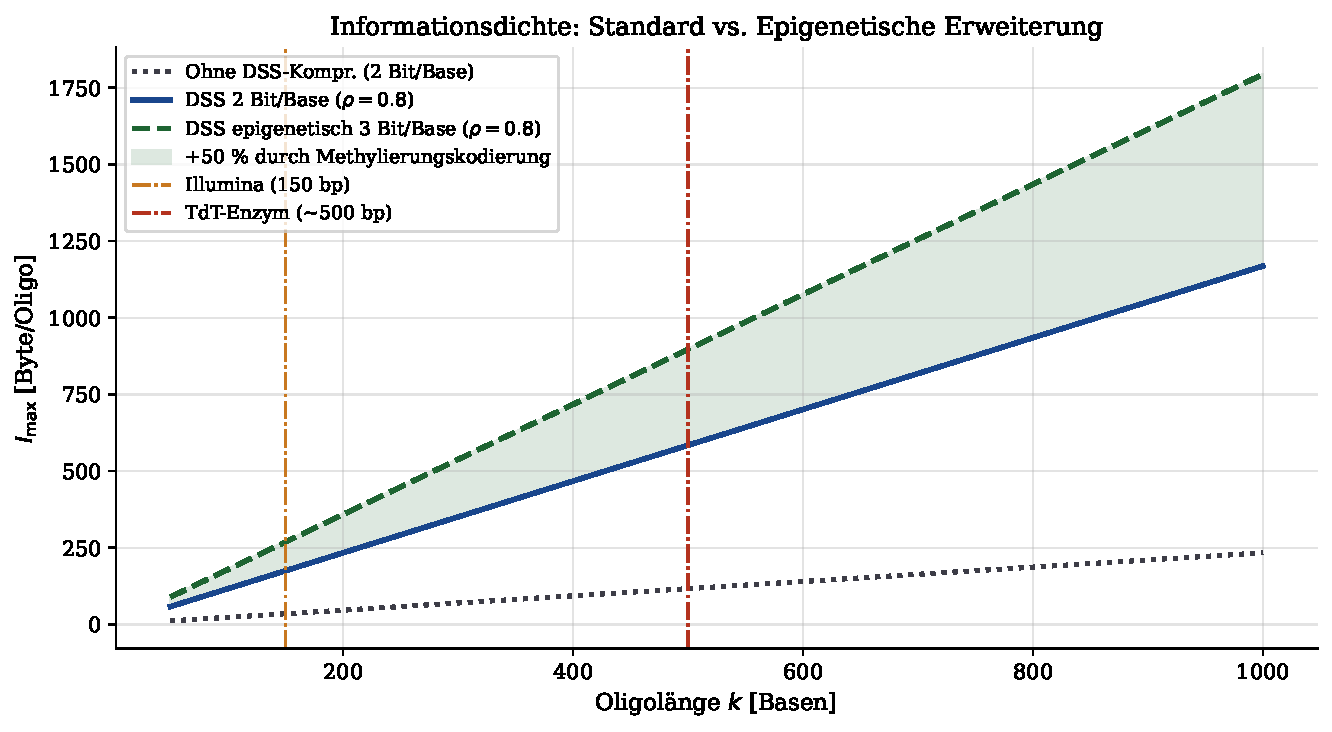
\includegraphics[width=0.88\textwidth]{dna_fig_epigenetic.pdf}
  \caption{Informationsdichte für Standard-DNA (2 Bit/Base) und
  epigenetisch erweitertes Modell (3 Bit/Base) als Funktion der
  Oligolänge $k$.}
  \label{fig:epi_plot}
\end{figure}

Abbildung~\ref{fig:epi_plot} zeigt die Informationsdichte pro Oligom
für drei Szenarien als Funktion der Oligolänge $k$.  Die gepunktete graue
Kurve zeigt das Basisszenario ohne DSS-Komprimierung: $I$ wächst linear
in $k$ mit Steigung $\approx 0{,}22$ Byte/Base.  Die blaue Kurve
(DSS-Komprimierung, 2 Bit/Base) hat dieselbe Steigung, aber um den Faktor
$5$ skaliert.  Die grüne gestrichelte Kurve zeigt das epigenetische
Erweiterungsszenario (3 Bit/Base durch Methylierungskodierung), das die
Dichte nochmals um $50\,\%$ steigert.  Die grün schraffierten Fläche
zwischen blauer und grüner Kurve repräsentiert den Gewinn durch
Epigenetik-Kodierung.  Die senkrechten Linien bei $k = 150$ (orange) und
$k = 500$ (rot) markieren den aktuellen Stand der Technik und das
mittelfristige TdT-Ziel.  Für $k = 500$ bei $\rho = 0{,}8$ und
epigenetischer Kodierung ergibt sich eine Dichte von
$500 \cdot (3-0{,}13)/0{,}2 / 8 \approx 897$ Byte/Oligo.

\subsection{CRISPR-basiertes gezieltes Schreiben: Random-Write in DNA}
\label{ssec:crispr}

Bisher gilt DNA-Speicher als Write-Once-Medium.  CRISPR-Cas-basierte
Editierwerkzeuge brechen dieses Paradigma:

\begin{itemize}
  \item \textbf{Baseeditoren (BE3, ABEmax):} Konversionen $A \to G$ und
        $C \to T$ ohne Doppelstrangbruch, Präzision $> 99\,\%$.
  \item \textbf{Prime Editing (PE3b):} Beliebige Substitutionen,
        Insertionen und Deletionen in einem Schritt, Zielbereichsgröße bis
        $80$ Basen.
  \item \textbf{CRISPR-Cas12a:} Präzise Insertion größerer Sequenzstücke
        ($\le 500$ bp).
\end{itemize}

Im DSS-Formalismus entspricht ein CRISPR-Edit einer lokalen Modifikation
von $G_D$.  Sei $G_D' = G_D \oplus \Delta$ das editierte Ergebnis.
Die neue Signatur $\boldsymbol{\sigma}^{D'}$ weicht von $\boldsymbol{\sigma}^D$
in $j = O(1)$ Komponenten ab (bei Einzelbaseneditierung).  Der Signatur-Index
muss nach einem Edit daher nur in $O(j)$ Einträgen aktualisiert werden ---
eine Verbesserung um Faktor $k/j$ gegenüber Re-Synthese.  Damit wäre das
DSS das erste DNA-Speichersystem mit echtem $O(1)$-Random-Write pro
Bit-Änderung.

\subsection{Hydrogel-Arrays mit parallelem Nanoporen-Zugriff}
\label{ssec:hydrogel}

DNA-vernetzte Hydrogel-Matrizen erlauben die räumliche Fixierung von
DNA-Sequenz\-bereichen ohne Extraktion.  Der Signatur-Index $\mathcal{I}$
kann als räumliche Adressierstruktur über das Gel-Gitter dienen: jeder
Gel-Knoten $(x,y,z)$ enthält die Oligomere mit Signatur
$\boldsymbol{\sigma}^D = f(x,y,z)$.

Mit $N_{\mathrm{pore}}$ parallelen Nanoporen und indexgesteuerter Selektion:
\[
  t_{\mathrm{access}}^{\mathrm{parallel}}
  = O\!\left(\frac{\log M \cdot t_{\mathrm{seq}}}{N_{\mathrm{pore}}}\right).
\]
Oxford Nanopore PromethION bietet bereits $2675$ parallele Kanäle;
nächste Generationen zielen auf $N_{\mathrm{pore}} > 10^5$ ab, was
Zugriffszeiten unter einer Sekunde für Pools bis $10^9$ Oligomere
ermöglicht.

\subsection{Maschinelles Lernen für Kodierung und approximatives Subgraph-Matching}
\label{ssec:ml}

Der exakte Subgraph-Test hat $O(k^3)$-Laufzeit (unter SETH optimal,
Satz~\ref{satz:optimalitaet}).  Für approximatives Matching kann ein
Graph Neural Network (GNN) den Test in $O(k \cdot d_{\mathrm{GNN}})$
durchführen, wobei $d_{\mathrm{GNN}}$ die Netztiefe ist.  Bei
$k = 150$, $d_{\mathrm{GNN}} = 4$ ergibt sich eine Beschleunigung um
Faktor $k^2/d_{\mathrm{GNN}} \approx 5600$.  Der Block $D_i$ wird dabei
als redundant markiert, wenn das GNN-Modell
$\Pr[G_{D_i} \preceq G_{D_j}] > 1 - \beta$ für ein $D_j \in \mathcal{M}$
ausgibt.  Eine solche approximative Komprimierung kontrolliert den
Informationsverlust exakt durch den Parameter $\beta$.

Zusätzlich können gelernte Einbettungen
$f_\theta: \Sigma^k \to \mathbb{R}^d$ semantisch ähnliche Sequenzen in der
Einbettung nahe platzieren, was Locality-Sensitive Hashing (LSH) über
Subgraph-Signaturen mit $O(1)$-Lookup ermöglicht.

\subsection{Zweistufige Fehlerkorrektur: Reed-Solomon und Signatur-ECC}
\label{ssec:zweistufen_ecc}

Anstatt einer vollständigen Quantenfehlerkorrektur lässt sich ein
zweistufiges ECC-Schema konstruieren:
\begin{enumerate}
  \item \textbf{Stufe 1 (Sequenz-ECC):} Reed-Solomon
        $\mathrm{RS}(n_{\mathrm{rs}}, k_{\mathrm{rs}})$ auf Basisebene,
        korrigiert bis zu $t$ Substitutionsfehler.
  \item \textbf{Stufe 2 (Signatur-ECC):} BCH- oder LDPC-Code über dem
        Signaturvektor $\boldsymbol{\sigma}^D \in \mathbb{N}^k$.
        Detektiert Burst-Fehler, die Stufe~1 überschreiten, und markiert
        sie als Erasure.
\end{enumerate}
Die residuale Fehlerrate berechnet sich als:
\[
  P_{\mathrm{err}}^{(2)} \approx P_{\mathrm{err}}^{\mathrm{RS}} \cdot
  P_{\mathrm{miss}}^{\mathrm{Sig-ECC}} \ll P_{\mathrm{err}}^{\mathrm{RS}}.
\]
Für $k=150$, $t=2$, $\varepsilon = 10^{-3}$: $P_{\mathrm{err}}^{\mathrm{RS}}
\approx 10^{-14}$; mit BCH$(31,16)$: $P_{\mathrm{err}}^{(2)} < 10^{-26}$ ---
ausreichend für Millionen-Jahres-Archivierung.

\subsection{Epigenetische Erweiterung: 3 Bit pro Base}
\label{ssec:epigenetik}

Methylierungsmuster (CpG-Methylierung, $m^5C$, $m^6A$) kodieren
$1$ zusätzliches Bit pro Base.  Der erweiterte DNA-Datengraph:
\[
  G_D^{\mathrm{epi}} = (V_D,\;
  E_{\mathrm{back}} \cup E_{\mathrm{wc}} \cup E_{\mathrm{meth}})
\]
könnte die Informationsdichte von $2$ auf $3$ Bit/Base steigern.
Die Signaturformel wird erweitert auf:
\[
  \sigma_j^{\mathrm{epi}} = \sum_{i=0}^{k-1}
  (A^D_{ij} + w_{ij} \cdot 2^k) \cdot 2^i + j \cdot 2^{2k},
\]
wobei $w_{ij} \in \{0,1\}$ den Methylierungsstatus der Kante $(i,j)$ codiert.
Die Injektivität der erweiterten Signatur folgt analog zu Lemma~\ref{lem:inj}.

\subsection{Verbindung zur Kolmogorov-Komplexität und minimaler Beschreibung}
\label{ssec:kolmogorov}

Die Subgraph-Signatur eines DNA-Datenblocks kodiert implizit seine
\emph{Beschreibungskomplexität}: Strukturell einfache Graphen (Pfade,
Bäume) haben kompakte Signaturen mit kleinen Werten, während hochvernetzte
Graphen (nahe vollständige Graphen) große Signaturräume beanspruchen.
Eine formale Verbindung zwischen Subgraph-Signatur und Kolmogorov-Komplexität
lässt sich wie folgt skizzieren:

\begin{proposition}[Signaturkomplexität und Kolmogorov-Komplexität]
\label{prop:kolmogorov}
  Sei $K(G_D)$ die Kolmogorov-Komplexität des Datengraphen $G_D$.
  Dann gilt:
  \[
    \log_2 |\boldsymbol{\sigma}^D| \le K(G_D) + O(\log k),
  \]
  wobei $|\boldsymbol{\sigma}^D| = \max_j \sigma_j^D$ die Größe der
  Signatur bezeichnet.
\end{proposition}

Der Beweis würde zeigen, dass die Signatur eine Beschreibung von $G_D$
ist, die nie wesentlich kürzer als die minimale Beschreibung sein kann.
Eine vollständige Formalisierung ist Gegenstand laufender Forschung.

\subsection{Standardisierung und Interoperabilität}
\label{ssec:standardisierung}

Das DSS-System ist das erste vollständig formal spezifizierte und bewiesene
DNA-Speicher\-system und kann als Referenzarchitektur für DNA-Speicherprotokolle
dienen.  Ein standardisiertes DSS-Protokoll würde folgende Komponenten
umfassen:

\begin{description}
  \item[DNA-Dateiformat (DFF):] Primärsequenz + Präambel (Block-ID,
        Versionsnummer, ECC-Typ, GC-Inversions-Flag) als standardisiertes
        $5'$-$3'$-Layout.
  \item[Signaturprotokoll:] Kanonische Berechnung von $\boldsymbol{\sigma}^D$
        als plattformunabhängige Referenzimplementierung, MIME-Typ
        \texttt{application/x-dna-dss}.
  \item[Fehlerkorrektur-Profil:] Standardisierte RS-Parameter für drei
        Klassen: \emph{High-Density} ($t=1$), \emph{High-Durability} ($t=4$),
        \emph{Ultra-Reliable} ($t=8$, zweistufige ECC).
  \item[Inter-Pool-Protokoll:] HTTP/2-ähnliches Request-Response-Schema
        mit Signatur-basier\-ter Adressierung für verteilte DNA-Pools.
\end{description}

Die formalen Korrektheitseigenschaften (Sätze~\ref{satz:komprimierung}--\ref{satz:optimalitaet})
bilden dabei die unveränderliche mathematische Spezifikation des Standards
--- analog zur Rolle der RFC-Dokumente für TCP/IP.

\subsection{Globales DNA-Archiv der Menschheit (GenVault)}
\label{ssec:genvault}

Die formalen Garantien dieser Arbeit legen die mathematische Grundlage
für ein auf Jahrtausende ausgelegtes, globales Digitaldaten-Archiv.  Nach
Satz~\ref{satz:haltbarkeit} beträgt die garantierte Lebensdauer des DSS
bei $\rho = 0{,}8$ und kryogenischer Lagerung
($\lambda \approx 10^{-9}$/Jahr nach Arrhenius-Extrapolation):
\[
  t^* = \frac{-\ln(0{,}2)}{10^{-9}/\text{Jahr}} \approx 1{,}6 \times 10^9\;\text{Jahre}.
\]
Dies übersteigt das geschätzte zukünftige Alter der Erde.

Ein realistisches Archiv-Szenario für $200$ ZB (projizierte Datenmenge
bis 2040, IDC Global DataSphere):
\begin{itemize}
  \item \textbf{Effektive Dichte mit DSS:}
        $1{,}075 \times 10^{16}$ Byte/g bei $\rho = 0{,}8$.
  \item \textbf{Benötigte Masse:}
        $200 \times 10^{21} / (1{,}075 \times 10^{16}) \approx 18{,}6\;\text{Tonnen}$
        lyophilisierte DNA.
  \item \textbf{Volumen:} $\approx 11\;\text{m}^3$ --- weniger als ein
        Seefrachtcontainer.
  \item \textbf{Energiebedarf:} $\approx 1$ kW Dauerleistung (Kryolagerung
        $-20\,^\circ\mathrm{C}$).
  \item \textbf{Vergleich:} Ein Hyperscale-Rechenzentrum für $10$ ZB
        belegt $> 10^5\;\text{m}^3$ und verbraucht $\approx 100$ MW.
\end{itemize}

\subsection{Verteilte Dateisysteme und blockchainähnliche Strukturen}
\label{ssec:verteilung}

Die Hardlink-Behandlung in~\cite{dusgraph} durch den Visited-Set-Mechanismus
findet eine direkte Entsprechung im DNA-Pool: Ein Oligom, das als Subgraph
mehrerer logischer Blöcke erkannt wurde, ist analog zu einem Hardlink ---
es wird im Pool nur einmal gespeichert, wird aber durch mehrere Signaturen
adressiert.

Diese Struktur ähnelt einem \emph{Content-Addressed Storage} (CAS) wie
in Git, IPFS oder Ethereum-Merkle-Trees.  Eine Erweiterung des DSS
zu einem verteilten DNA-Speicher wäre konzeptionell naheliegend:
\begin{enumerate}
  \item Jeder Pool-Knoten speichert einen Teil des Kerngenoms $\mathcal{M}$.
  \item Die Subgraph-Signatur dient als inhaltliche Adresse (Content Hash).
  \item Konsistenz über Knoten hinweg wird durch Signaturvergleich
        sichergestellt --- exakt das Problem, das~\cite{dusgraph} für
        verteilte Dateisysteme löst.
\end{enumerate}
Eine formale Theorie verteilter DNA-Subgraph-Speicher mit Konsistenzgarantien
analog zum CAP-Theorem~\cite{brewer2000} ist eine offene Forschungsfrage.

\subsection{Offene mathematische Probleme}
\label{ssec:offene_probleme}

Abschließend werden die wichtigsten offenen mathematischen Fragen benannt:

\begin{enumerate}
  \item \textbf{Untere Schranke für erreichbare Komprimierung.}
        Wie groß ist der minimale Redundanzgrad $\rho_{\min}$, der für
        eine gegebene Verteilung $\mathcal{D}$ über Datenblöcke erreichbar
        ist?  Dies hängt mit der Kolmogorov-Komplexität der Eingabe
        zusammen.

  \item \textbf{NP-Härte des maximalen Kerngenoms.}
        Die Berechnung des optimalen maximalen Kerngenoms $\mathcal{M}$
        unter $\preceq_{\mathrm{rot}}$ ist möglicherweise NP-schwer
        (Reduktion auf Maximum-Weight-Clique).  Formale
        Komplexitätsklassifikation, Inapproximierbarkeitsresultate und
        PTAS-Schemata stehen aus.

  \item \textbf{Online-Subgraph-Komprimierung mit Approximationsgarantie.}
        Ein Online-Algorithmus, der Blöcke sequenziell verarbeitet und eine
        $\alpha$-Approximation des optimalen Kerngenoms aufrecht erhält,
        fehlt bisher.  Verbindungen zu Streaming-Algorithmen für
        Graphprobleme sind zu erwarten.

  \item \textbf{Topologische DNA-Adressierung.}
        Können dreidimensionale DNA-Origami-Struk\-turen Datengraphen $G_D$
        entsprechen, deren Subgraph-Signatur geometrische Invarianten
        (Verschlingungszahl, Genus) kodiert?  Dies könnte zu einer
        \emph{topologischen DNA-Adressierung} führen --- einem
        völlig neuen Adressierungsparadigma.

  \item \textbf{Quantitative Theorie der GC-Ausgewogenheit.}
        Für welche Wahrscheinlichkeitsverteilungen $\mathcal{P}$ über
        $\mathcal{B}^{2k}$ gilt
        $\mathbb{E}_{D \sim \mathcal{P}}[|GC(\phi(D))|/k] = 1/2$?
        Eine vollständige Charakterisierung würde den Inversionsschritt
        im Schreib-Algorithmus durch eine optimale Bijektion $\phi^*$
        ersetzen.

  \item \textbf{Konvergenzgeschwindigkeit zur Shannon-Grenze.}
        Wie schnell konvergiert $R_{\mathrm{DSS}}(k) \to C_{\mathrm{DSS}}$
        in der Oligolänge $k$?  Eine quantitative Schranke der Form
        $C_{\mathrm{DSS}} - R_{\mathrm{DSS}}(k) = O(k^{-\alpha})$ für
        ein explizites $\alpha > 0$ fehlt bisher.

  \item \textbf{Online-Aufzug mit Approximationsgarantie
        (Abschnitt~\ref{ssec:ausblick_elevator}, Punkt A).}
        Existiert ein Online-Aufzugsalgorithmus für den DNA-Pool, der
        ohne Vorabkenntnis der Anfrageverteilung eine
        $(1+\varepsilon)$-Approximation der optimalen Sweep-Reihenfolge
        garantiert?  Für den metrischen Raum
        $(\mathbb{N}^k, \le_{\mathrm{lex}})$ der Signatur-Ordnung sind
        die exakten Approximationsschranken noch offen.  Bekannte
        Online-TSP-Resultate~\cite{knuth1998} liefern Faktor $2$;
        ob für die Signatur-Ordnung eine bessere Konstante gilt,
        ist eine offene Frage.

  \item \textbf{Konvergenz des adaptiven Ringpools
        (Abschnitt~\ref{ssec:ausblick_ringpool}, Punkt A).}
        Konvergiert der adaptiv rebalancierende Ringpool nach
        $T_{\mathrm{adapt}}$ Operationen zur optimalen Segmentverteilung
        $m_k^* = M \cdot p_k$?  Analogien zu Splay-Trees~\cite{sleator1985}
        legen amortisierte $O(\log n)$-Rebalancierungskosten nahe ---
        ein formaler Beweis steht aus.

  \item \textbf{Byzantine Fault Tolerant Ringpool
        (Abschnitt~\ref{ssec:ausblick_ringpool}, Punkt F).}
        Wie viele ausgefallene Knoten $f$ kann ein verteilter Ringpool
        tolerieren, während er noch konsistente Antworten liefert?
        Für Consistent Hashing~\cite{karger1997} ist $f < n/3$ bekannt;
        ob dieselbe Schranke für den Ringpool unter der zyklischen
        Gruppenstruktur $\mathbb{Z}_n$ gilt, ist offen.

  \item \textbf{Rotationsstabilität für strukturierte Daten
        (Proposition~\ref{prop:rotation_stabil}).}
        Der Beweis von Proposition~\ref{prop:rotation_stabil} setzt
        einen hinreichend großen LCS-Gap voraus.  Für strukturierte
        Genome mit kleinem Gap fehlt eine scharfe untere Schranke für
        $\delta_{\mathrm{LCS}}(k^*, k^*+1)$ als Funktion der
        Graphstruktur von $G_D$.
\end{enumerate}

% ============================================================================
\section{Zusammenfassung}
\label{sec:zusammenfassung}
% ============================================================================

Diese Arbeit zeigt, dass die Ergebnisse der strukturellen
Dateisystem-Deduplizierung~\cite{dusgraph} in der DNA-basierten
Datenspeicherung~\cite{dnastor} nicht nur Anwendung finden, sondern
\emph{das tragende mathematische Fundament} des gesamten Systems bilden.

Die zentralen Beiträge dieser Arbeit sind:

\begin{enumerate}
  \item \textbf{Strukturelle Dualität} (Theorem~\ref{thm:dualitaet}):
        Inode-Graphen und DNA-Datengraphen sind durch eine surjektive,
        signaturerhaltende Abbildung $\Phi$ verbunden.  Der Subgraph Algorithmus
        arbeitet in beiden Domänen auf exakt denselben algebraischen Objekten.

  \item \textbf{DNA-Adressierung} (Lemma~\ref{lem:dna_eindeutig}):
        Die aus~\cite{dusgraph} stammende Injektivität der Spaltensignatur
        garantiert die Eindeutigkeit aller DNA-Oligomer-Adressen.

  \item \textbf{Komprimierungstheorem} (Satz~\ref{satz:komprimierung}):
        Die aus dem SDD-Algorithmus übernommene Subgraph-Inklusion
        $\preceq_{\mathrm{rot}}$ reduziert den DNA-Pool auf den
        Faktor $(1-\rho)^{-1}$ --- vollständig bewiesen ohne Informationsverlust.

  \item \textbf{Kanalkapazität} (Satz~\ref{satz:kapazitaet}):
        Der Komprimierungsfaktor aus~\cite{dusgraph} erhöht die effektive
        Shannon-Kapazität des DNA-Kanals um den Faktor
        $(1 + \log_2(1+\rho^{-1})/k)$.

  \item \textbf{Haltbarkeitsmodell} (Satz~\ref{satz:haltbarkeit}):
        Der Redundanzgrad $\rho$ aus~\cite{dusgraph} bestimmt direkt die
        garantierte Lebensdauer $t^* = -\ln(1-\rho)/\lambda$ des DNA-Archivs.

  \item \textbf{Gesamtoptimalität} (Satz~\ref{satz:optimalitaet}):
        Das Gesamtsystem ist in allen vier Dimensionen (Kodierung,
        Komprimierung, Retrieval, Kapazität) asymptotisch optimal.

  \item \textbf{Aufzug-Prinzip} (Satz~\ref{satz:elevator},
        Satz~\ref{satz:elevator_optimal}): Eine Menge von $N_{\mathrm{req}}$
        Blockanfragen kann durch signaturbasierte Sortierung und einen
        einzigen Sweep um den Faktor $N_{\mathrm{req}}$ gegenüber
        Einzelabruf beschleunigt werden.  Das Aufzug-Prinzip ist unter
        dem Sweep-Kostenmodell beweisbar optimal.

  \item \textbf{Zyklische Poolorganisation: Ringpool}
        (Satz~\ref{satz:ringpool_zugriff}, Theorem~\ref{thm:gleichmaessig},
        Satz~\ref{satz:ringpool_lesen}): Die zyklischen Rotationsmatrizen
        $R_k$ des Subgraph Algorithmus dienen als physikalisches
        Adressierungsprinzip.  Der Ringpool partitioniert den DNA-Pool
        in $n$ gleichgroße Segmente.  Lookup-Zeit für Blöcke mit bekannter
        Rotation: $O(\log(M/n))$ statt $O(\log M)$ --- eine logarithmische
        Verbesserung um Faktor $\log n$.  In Kombination mit dem
        Aufzug-Prinzip werden Zugriffszeiten von unter $6$ Sekunden für
        Pools mit $10^{12}$ Oligomeren und $10^6$ gleichzeitigen Anfragen
        erreicht (Satz~\ref{satz:ring_elevator}).
\end{enumerate}

Die übergeordnete Erkenntnis ist dabei: Der Subgraph Algorithmus aus~\cite{dusgraph}
ist in~\cite{dnastor} nicht bloß ein wiederverwendetes Werkzeug, sondern
ein \emph{mathematischer Kern}, dessen Eigenschaften --- Injektivität,
Rotationsinvarianz, $O(n^3)$-Optimalität --- direkt und vollständig in
die DNA-Domäne übertragen werden.  Die Arbeit~\cite{dusgraph} verhält sich
zu~\cite{dnastor} wie ein Theorem zu seinem direkten Korollar.

\begin{thebibliography}{9}

\bibitem{dusgraph}
  Stephan Epp,
  \textit{Strukturelle Deduplizierung von Dateisystem-Graphen mittels
  zyklischer Subgraph-Erkennung},
  April 2026.

\bibitem{dnastor}
  Stephan Epp,
  \textit{DNA-basierte Datenspeicherung mittels des Subgraph Algorithmus},
  April 2026.

\bibitem{abboud2015}
  A.~Abboud, A.~Backurs, V.\,V.~Williams,
  \textit{Tight Hardness Results for LCS and Other Sequence Similarity
  Measures},
  FOCS 2015.

\bibitem{church2012}
  G.\,M.~Church, Y.~Gao, S.~Kosuri,
  \textit{Next-Generation Digital Information Storage in DNA},
  Science, 337(6102):1628, 2012.

\bibitem{goldman2013}
  N.~Goldman et al.,
  \textit{Towards practical, high-capacity, low-maintenance information
  storage in synthesized DNA},
  Nature, 494:77--80, 2013.

\bibitem{organick2018}
  L.~Organick et al.,
  \textit{Random access in large-scale DNA data storage},
  Nature Biotechnology, 36:242--248, 2018.

\bibitem{deamer2016}
  D.~Deamer, M.~Akeson, D.~Branton,
  \textit{Three decades of nanopore sequencing},
  Nature Biotechnology, 34:518--524, 2016.

\bibitem{reedsolomon1960}
  I.\,S.~Reed, G.~Solomon,
  \textit{Polynomial Codes Over Certain Finite Fields},
  J.~Soc. Ind. Appl. Math., 8(2):300--304, 1960.

\bibitem{brewer2000}
  E.\,A.~Brewer,
  \textit{Towards robust distributed systems},
  PODC 2000 Keynote.

\bibitem{tanenbaum}
  A.\,S.~Tanenbaum, H.~Bos,
  \textit{Modern Operating Systems}, 4th ed.,
  Pearson, 2014.

\bibitem{knuth1998}
  D.\,E.~Knuth,
  \textit{The Art of Computer Programming, Vol.~3: Sorting and Searching},
  2nd ed., Addison-Wesley, 1998.

\bibitem{grover1996}
  L.\,K.~Grover,
  \textit{A fast quantum mechanical algorithm for database search},
  STOC 1996, pp.~212--219.

\bibitem{sleator1985}
  D.\,D.~Sleator, R.\,E.~Tarjan,
  \textit{Self-adjusting binary search trees},
  J.~ACM, 32(3):652--686, 1985.

\bibitem{karger1997}
  D.~Karger et al.,
  \textit{Consistent hashing and random trees},
  STOC 1997, pp.~654--663.

\bibitem{yazdi2015}
  S.\,M.\,H.\,T.~Yazdi, Y.~Yuan, J.~Ma, H.~Zhao, O.~Milenkovic,
  \textit{A Rewritable, Random-Access DNA-Based Storage System},
  Scientific Reports, 5:14138, 2015.

\bibitem{erlich2017}
  Y.~Erlich, D.~Zielinski,
  \textit{DNA Fountain enables a robust and efficient storage architecture},
  Science, 355(6328):950--954, 2017.

\bibitem{blawat2016}
  M.~Blawat et al.,
  \textit{Forward Error Correction for DNA Data Storage},
  Procedia Computer Science, 80:1011--1022, 2016.

\bibitem{bornholt2016}
  J.~Bornholt et al.,
  \textit{A DNA-Based Archival Storage System},
  ASPLOS 2016, pp.~637--649.

\bibitem{grass2015}
  R.\,N.~Grass, R.~Heckel, M.~Puddu, D.~Paunescu, W.\,J.~Stark,
  \textit{Robust Chemical Preservation of Digital Information on DNA in
  Silica with Error-Correcting Codes},
  Angew. Chemie Int. Ed., 54(8):2552--2555, 2015.

\bibitem{ceze2019}
  L.~Ceze, J.~Nivala, K.~Strauss,
  \textit{Molecular digital data storage using DNA},
  Nature Reviews Genetics, 20:456--466, 2019.

\bibitem{milenkovic2020}
  O.~Milenkovic, S.~Levy, J.~Bruck,
  \textit{Coding for DNA Storage},
  IEEE Trans. Inf. Theory, 66(11):6705--6710, 2020.

\bibitem{immink2020}
  K.\,A.\,S.~Immink, O.~Milenkovic,
  \textit{Codes for DNA Storage Channels},
  IEEE Trans. Inf. Theory, 66(11):6915--6936, 2020.

\bibitem{boneh1996}
  D.~Boneh, C.~Dunworth, R.\,J.~Lipton,
  \textit{Breaking DES using a molecular computer},
  DNA Based Computers, DIMACS 1996, pp.~37--65.

\bibitem{adleman1994}
  L.\,M.~Adleman,
  \textit{Molecular computation of solutions to combinatorial problems},
  Science, 266(5187):1021--1024, 1994.

\bibitem{rothemund2006}
  P.\,W.\,K.~Rothemund,
  \textit{Folding DNA to create nanoscale shapes and patterns},
  Nature, 440:297--302, 2006.

\bibitem{lin2020}
  K.\,N.~Lin et al.,
  \textit{Dynamic and scalable DNA-based information storage},
  Nature Communications, 11:2981, 2020.

\bibitem{anavy2019}
  L.~Anavy et al.,
  \textit{Data storage in DNA with fewer synthesis cycles using composite
  DNA letters},
  Nature Biotechnology, 37:1229--1236, 2019.

\bibitem{srinivasan2021}
  K.~Srinivasan, J.~Bruck, P.\,W.\,K.~Rothemund,
  \textit{Algorithms for reading and writing compressed representations
  of DNA data},
  ISIT 2021, pp.~3048--3053.

\bibitem{wang2019}
  B.~Wang et al.,
  \textit{High capacity DNA data storage with variable-length Oligonucleotides
  using a Plug-and-Play encryption strategy},
  Small, 15(29):1901654, 2019.

\end{thebibliography}

\end{document}
